%!TEX root = ddoti.tex

\chapter{Instrument}

\section{Maintenance Procedure}

\subsection{Changing a Detector}

The detectors are attached to an adapter which is in turn attached to a mounting ring on the telescope corrector plate. The mounting ring appears to be held against rotation by friction. Thus, care must be taken to avoid placing a torque on the mounting ring when manipulating the detector and adapter.

\subsubsection{Safety Considerations}

\safety{Use a harness, line, and helmet when you work on the platform or balconies.}

\safety{Under no circumstances ascend to the platform or balconies if the enclosure is in remote mode as the enclosure can close without warning.}

\subsubsection{Requirements}

You will need:

\begin{itemize}
\item Two persons.
\item The key to the shed (see \S\ref{section:shed-key}).
\item Metric hex keys (specifically, 2 and 2.5 mm)
\item Wire cutters
\item Cable ties
\item A spirit level
\end{itemize}

\subsubsection{Procedure}

\begin{enumerate}
\item
Use appropriate safety equipment: harnesses, lines, and helmets. These are found in the shed.

\item
Move the enclosure controller mode selector switch to “LOCAL”.

\item If the weather permits, open the enclosure to 60 $\deg$.

Set the angle selector switch to the 60 $\deg$ and then press and hold the “OPEN” button until the green light goes out.

\item Ascend to the platform.

\begin{figure*}
\begin{center}
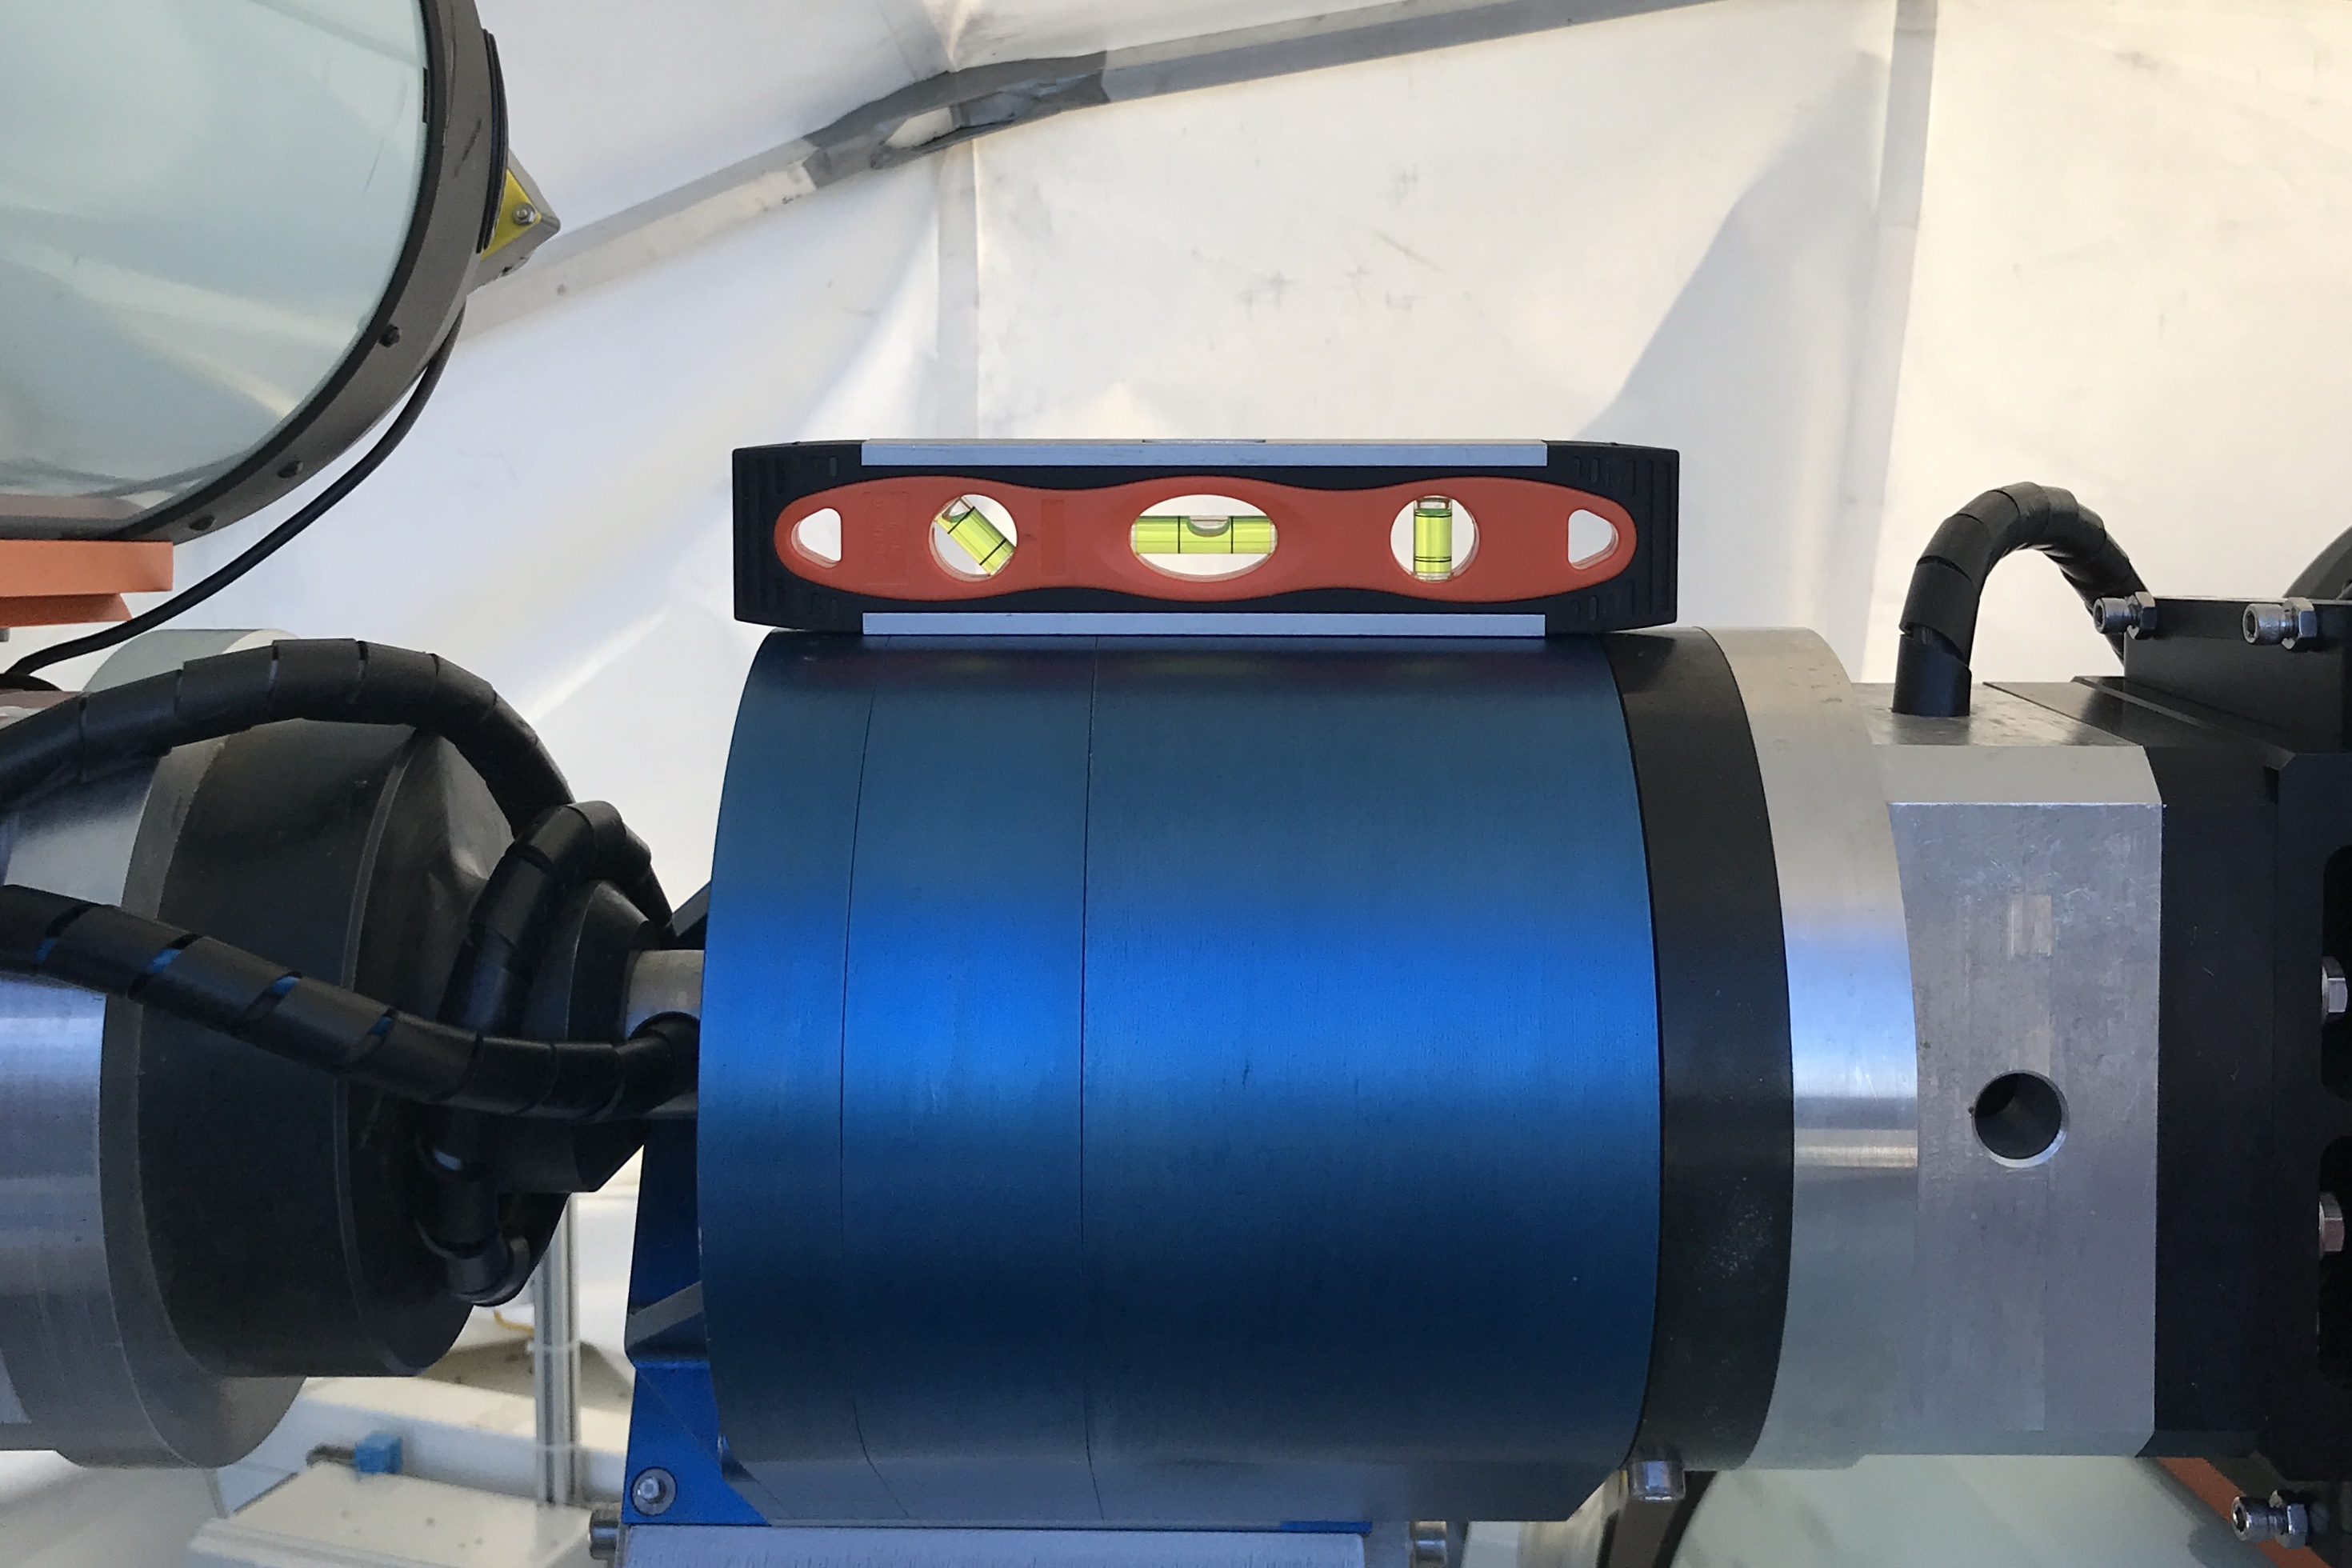
\includegraphics[width=0.7\linewidth]{figures/instrument-ddoti-mount-level.jpg}
\end{center}
\caption{Using the spirit level to make sure that the declination axis is horizontal.}
\label{figure:instrument-ddoti-mount-level}
\end{figure*}

\item Point the telescope to the northern horizon. Verify that the declination axis is horizontal using the spirit level. See Figure~\ref{figure:instrument-ddoti-mount-level}.

While supporting the telescopes using one of the handles on the primary mirror cells, push the button on the mount to release the brake. Move the telescopes to point at the northern horizon. Then use the spirit level to make sure that the declination axis is horizontal.

\begin{figure*}
\begin{center}
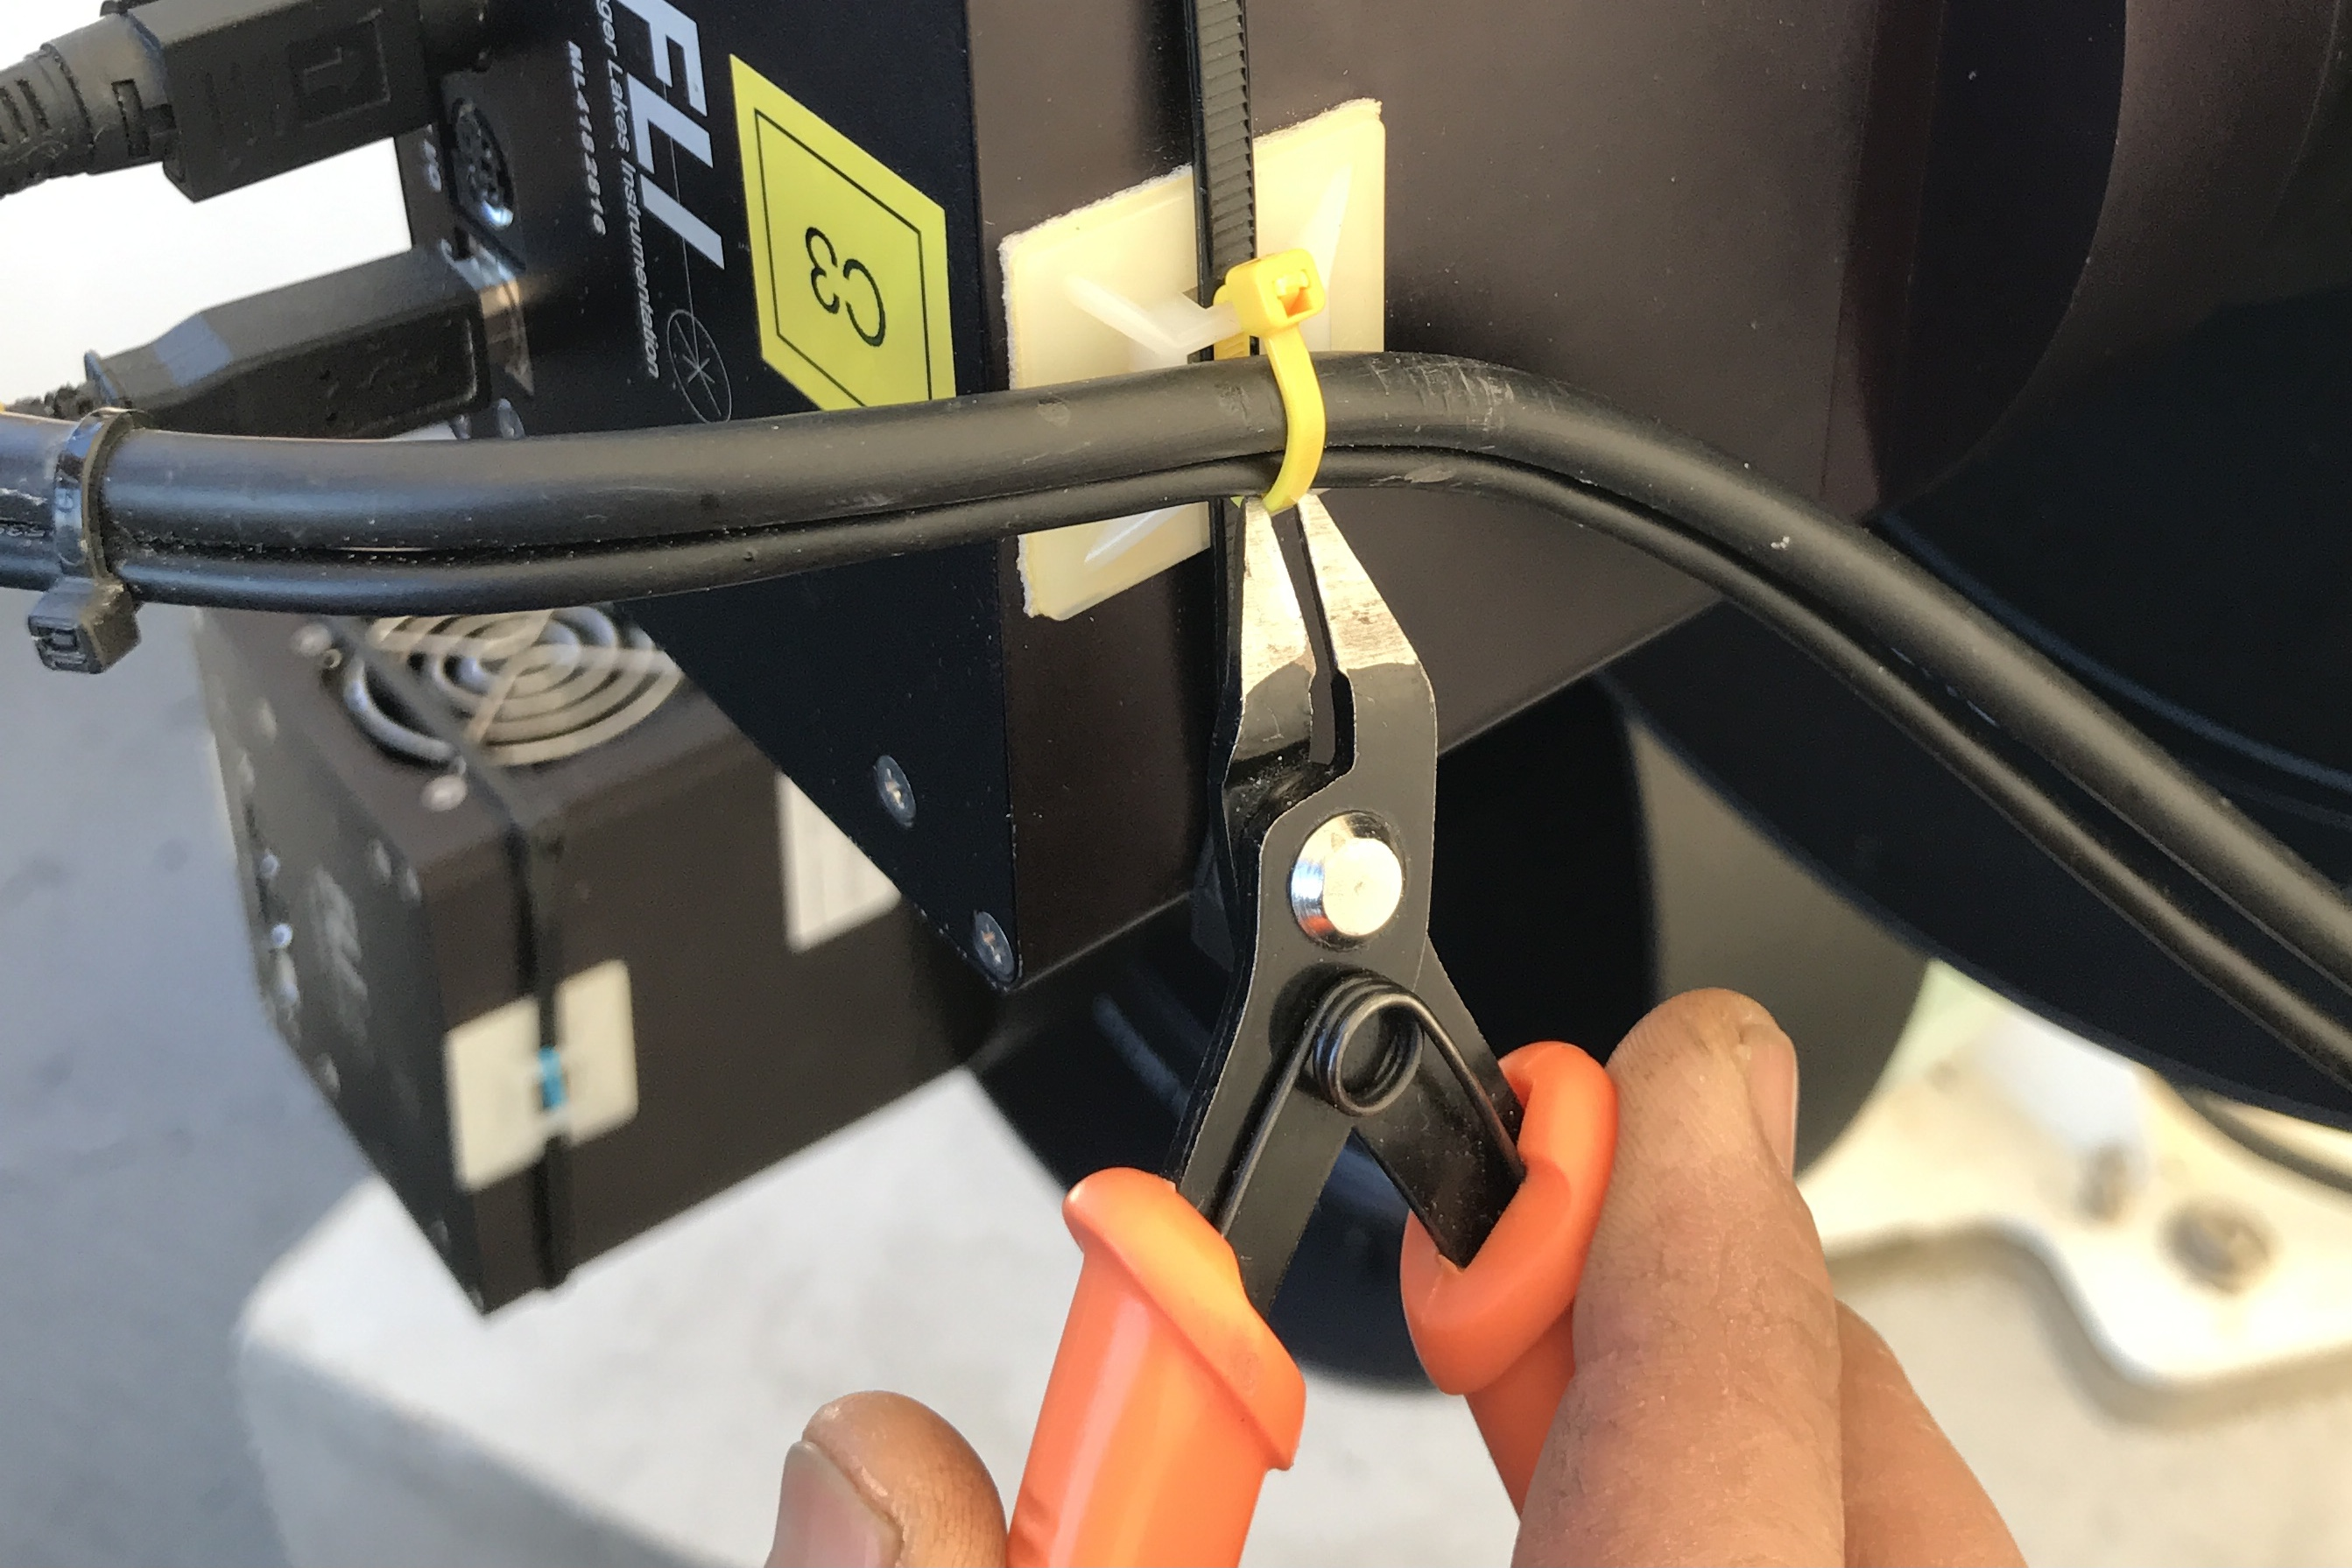
\includegraphics[width=0.7\linewidth]{figures/instrument-ddoti-cutting-cable-ties.jpg}
\end{center}
\caption{Cutting the cable ties of the detector to be replaced.}
\label{figure:instrument-ddoti-cutting-cable-ties}
\end{figure*}

\item Cut the cable ties on the detector to be replaced. See Figure~\ref{figure:instrument-ddoti-cutting-cable-ties}.

\begin{figure*}
\begin{center}
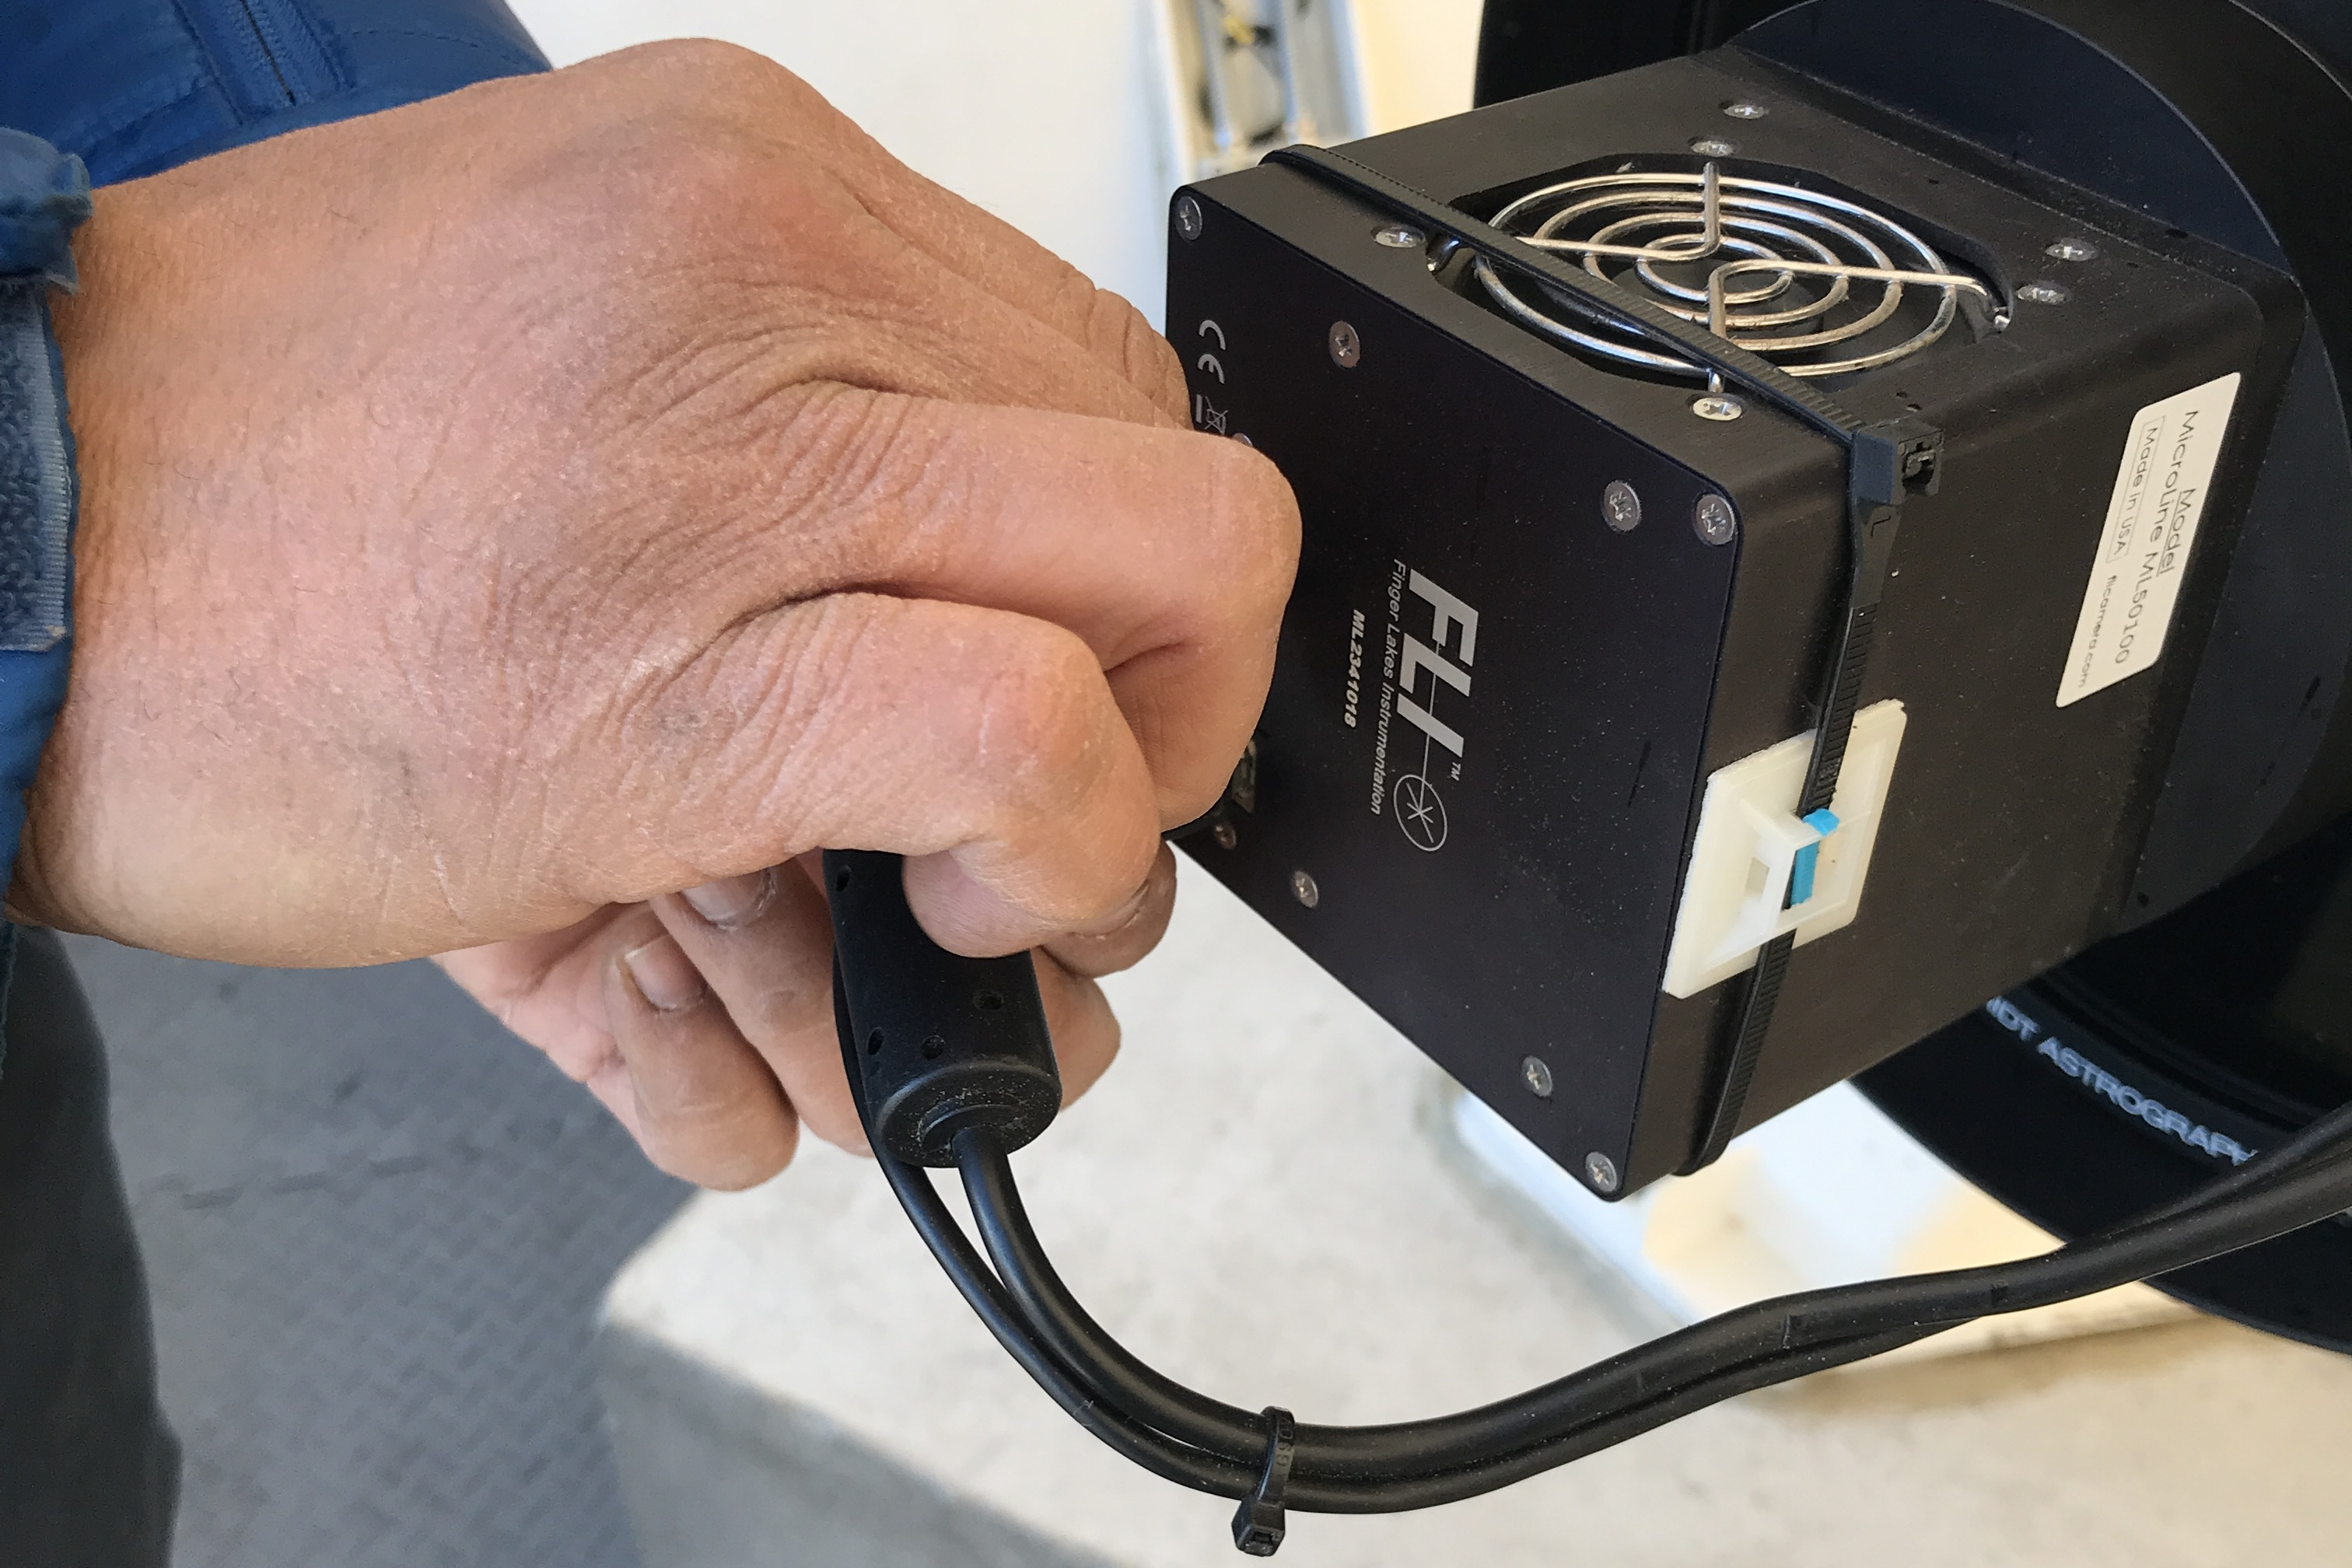
\includegraphics[width=0.7\linewidth]{figures/instrument-ddoti-removing-cables.jpg}
\end{center}
\caption{Removing the cables from the detector to be replaced. Be careful not to apply a torque on the detector.}
\label{figure:instrument-ddoti-removing-cables}
\end{figure*}

\item Gently remove the USB and power cables. Support the detector to avoid placing a torque on the mounting ring. See Figure~\ref{figure:instrument-ddoti-removing-cables}.

\begin{figure*}
\begin{center}
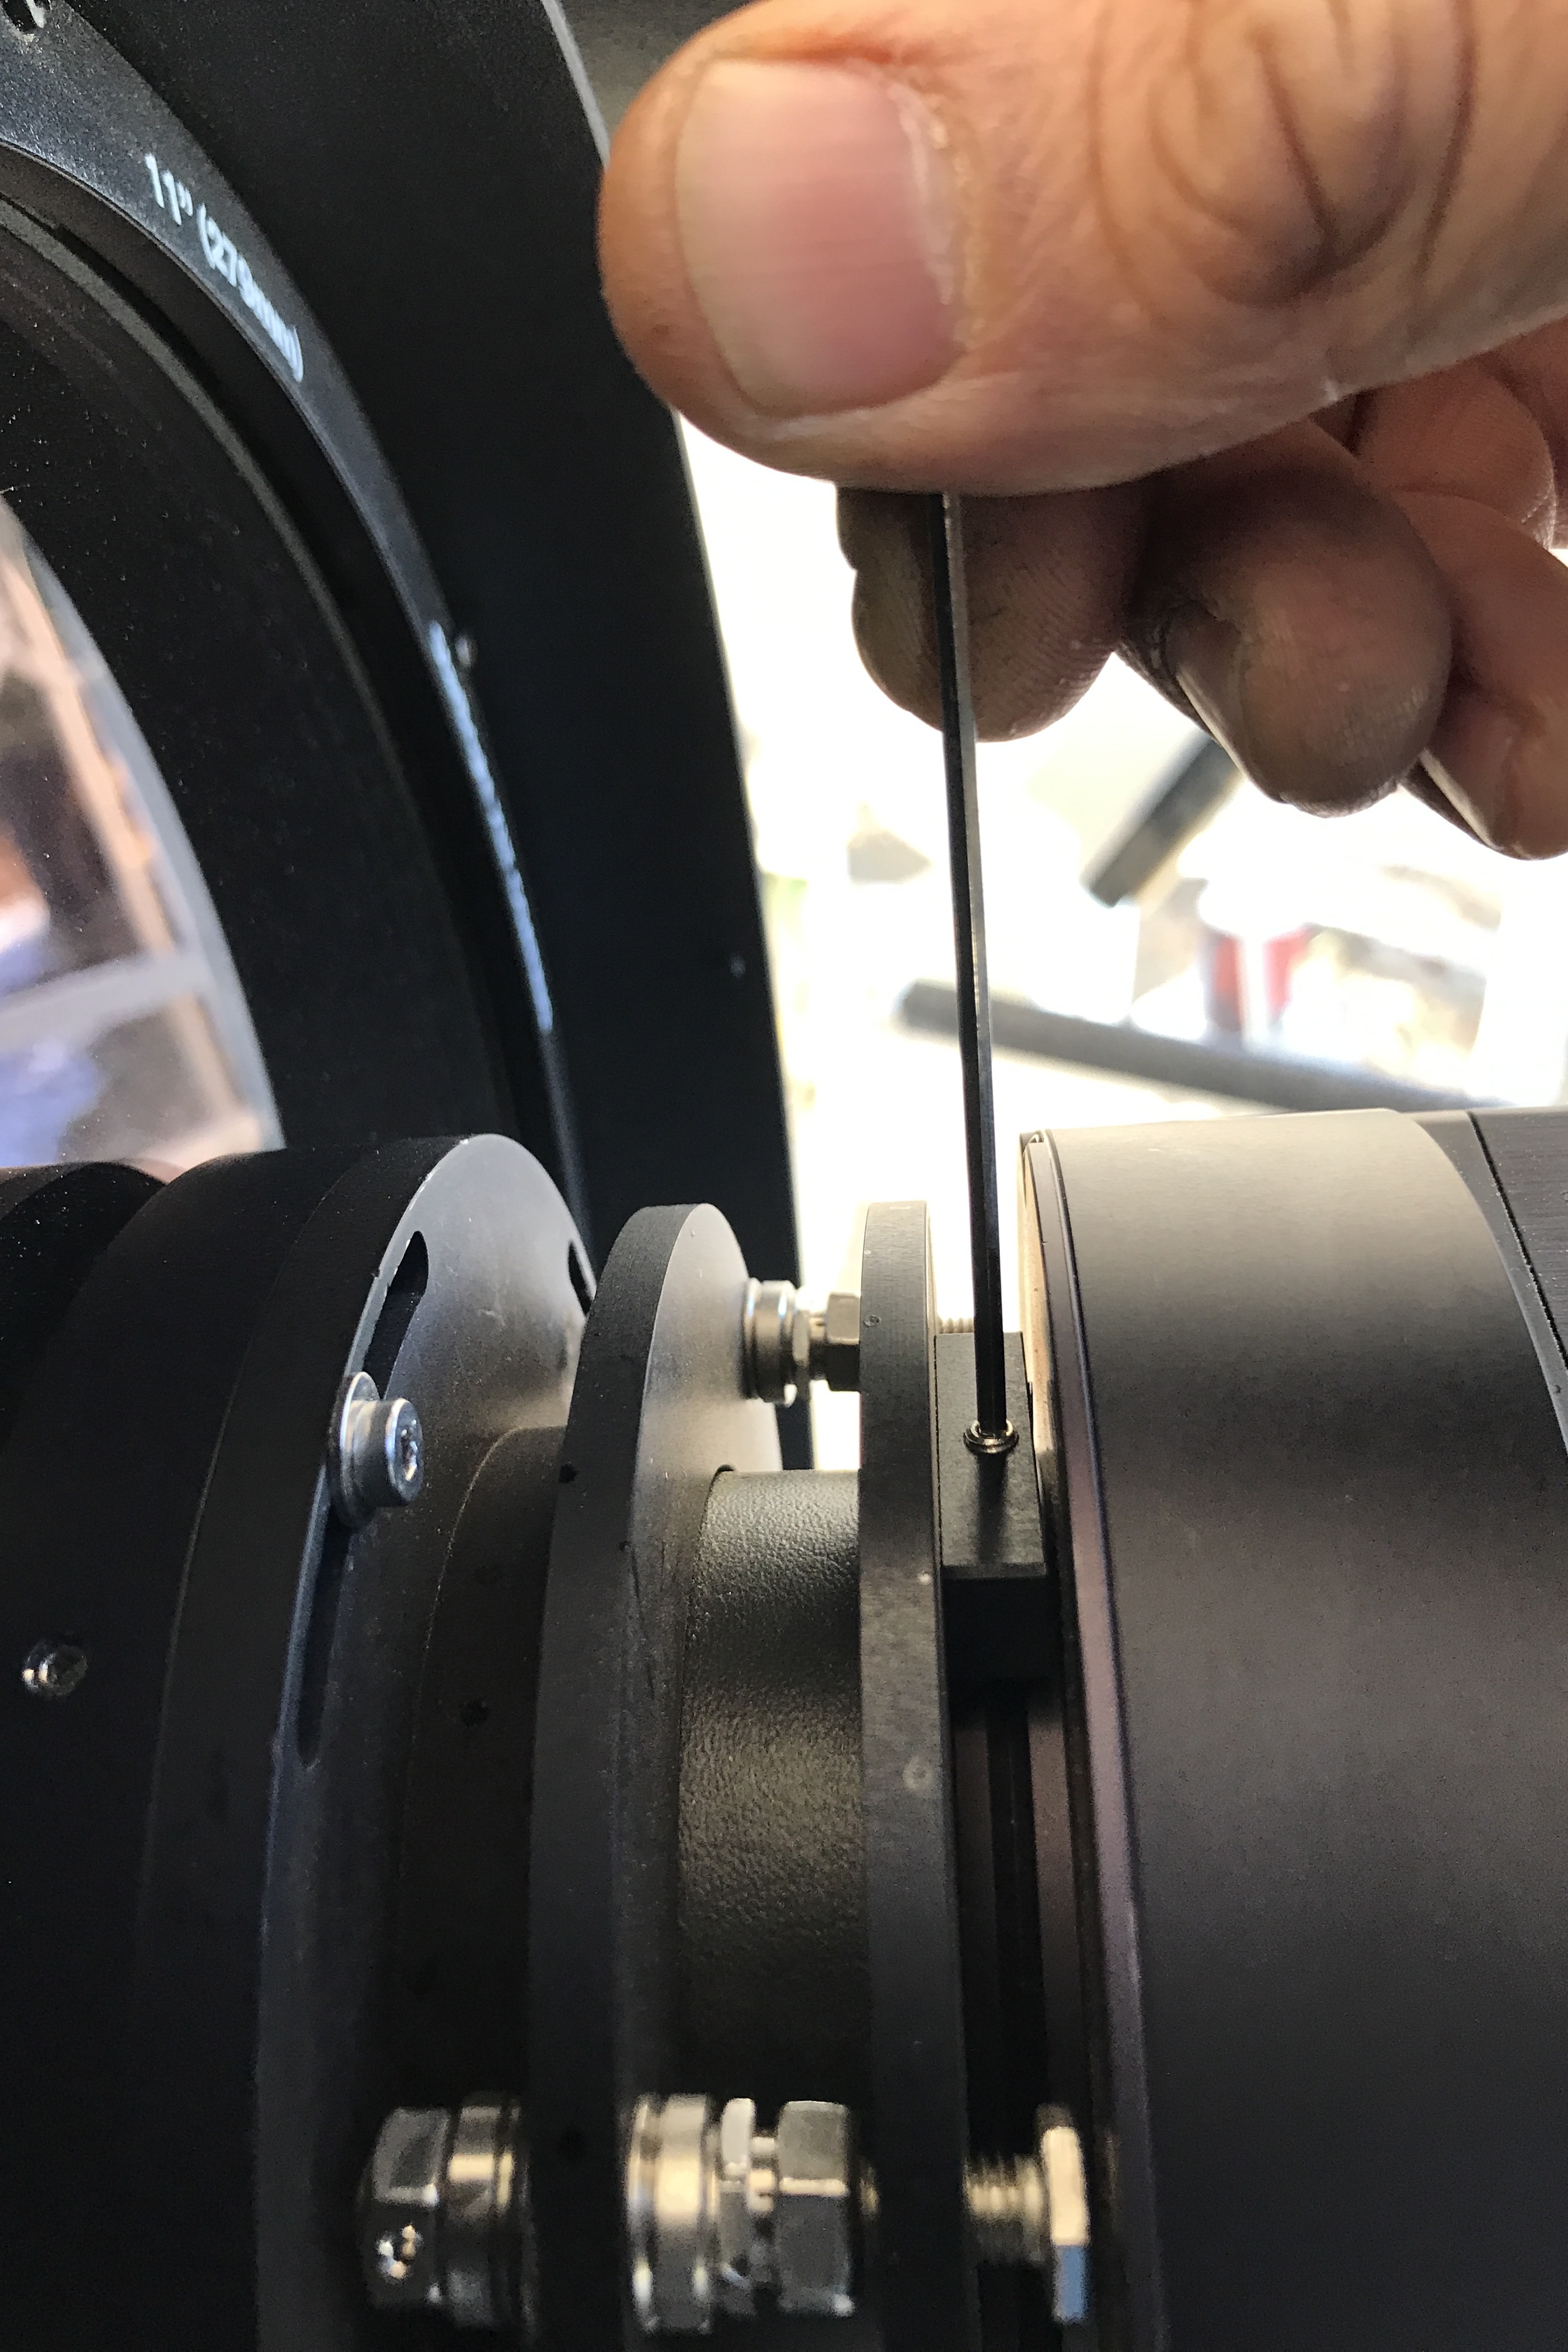
\includegraphics[height=0.7\linewidth]{figures/instrument-ddoti-slackening-grub-screw.jpg}
\end{center}
\caption{Slackening the grub screw.}
\label{figure:instrument-ddoti-slackening-grub-screw}
\end{figure*}

\item Using a 2 mm hex key, gently slacken the grub screw that stops the detector from rotating in its adapter. Support the detector to avoid placing a torque on the mounting ring. See Figure~\ref{figure:instrument-ddoti-slackening-grub-screw}.

\begin{figure*}
\begin{center}
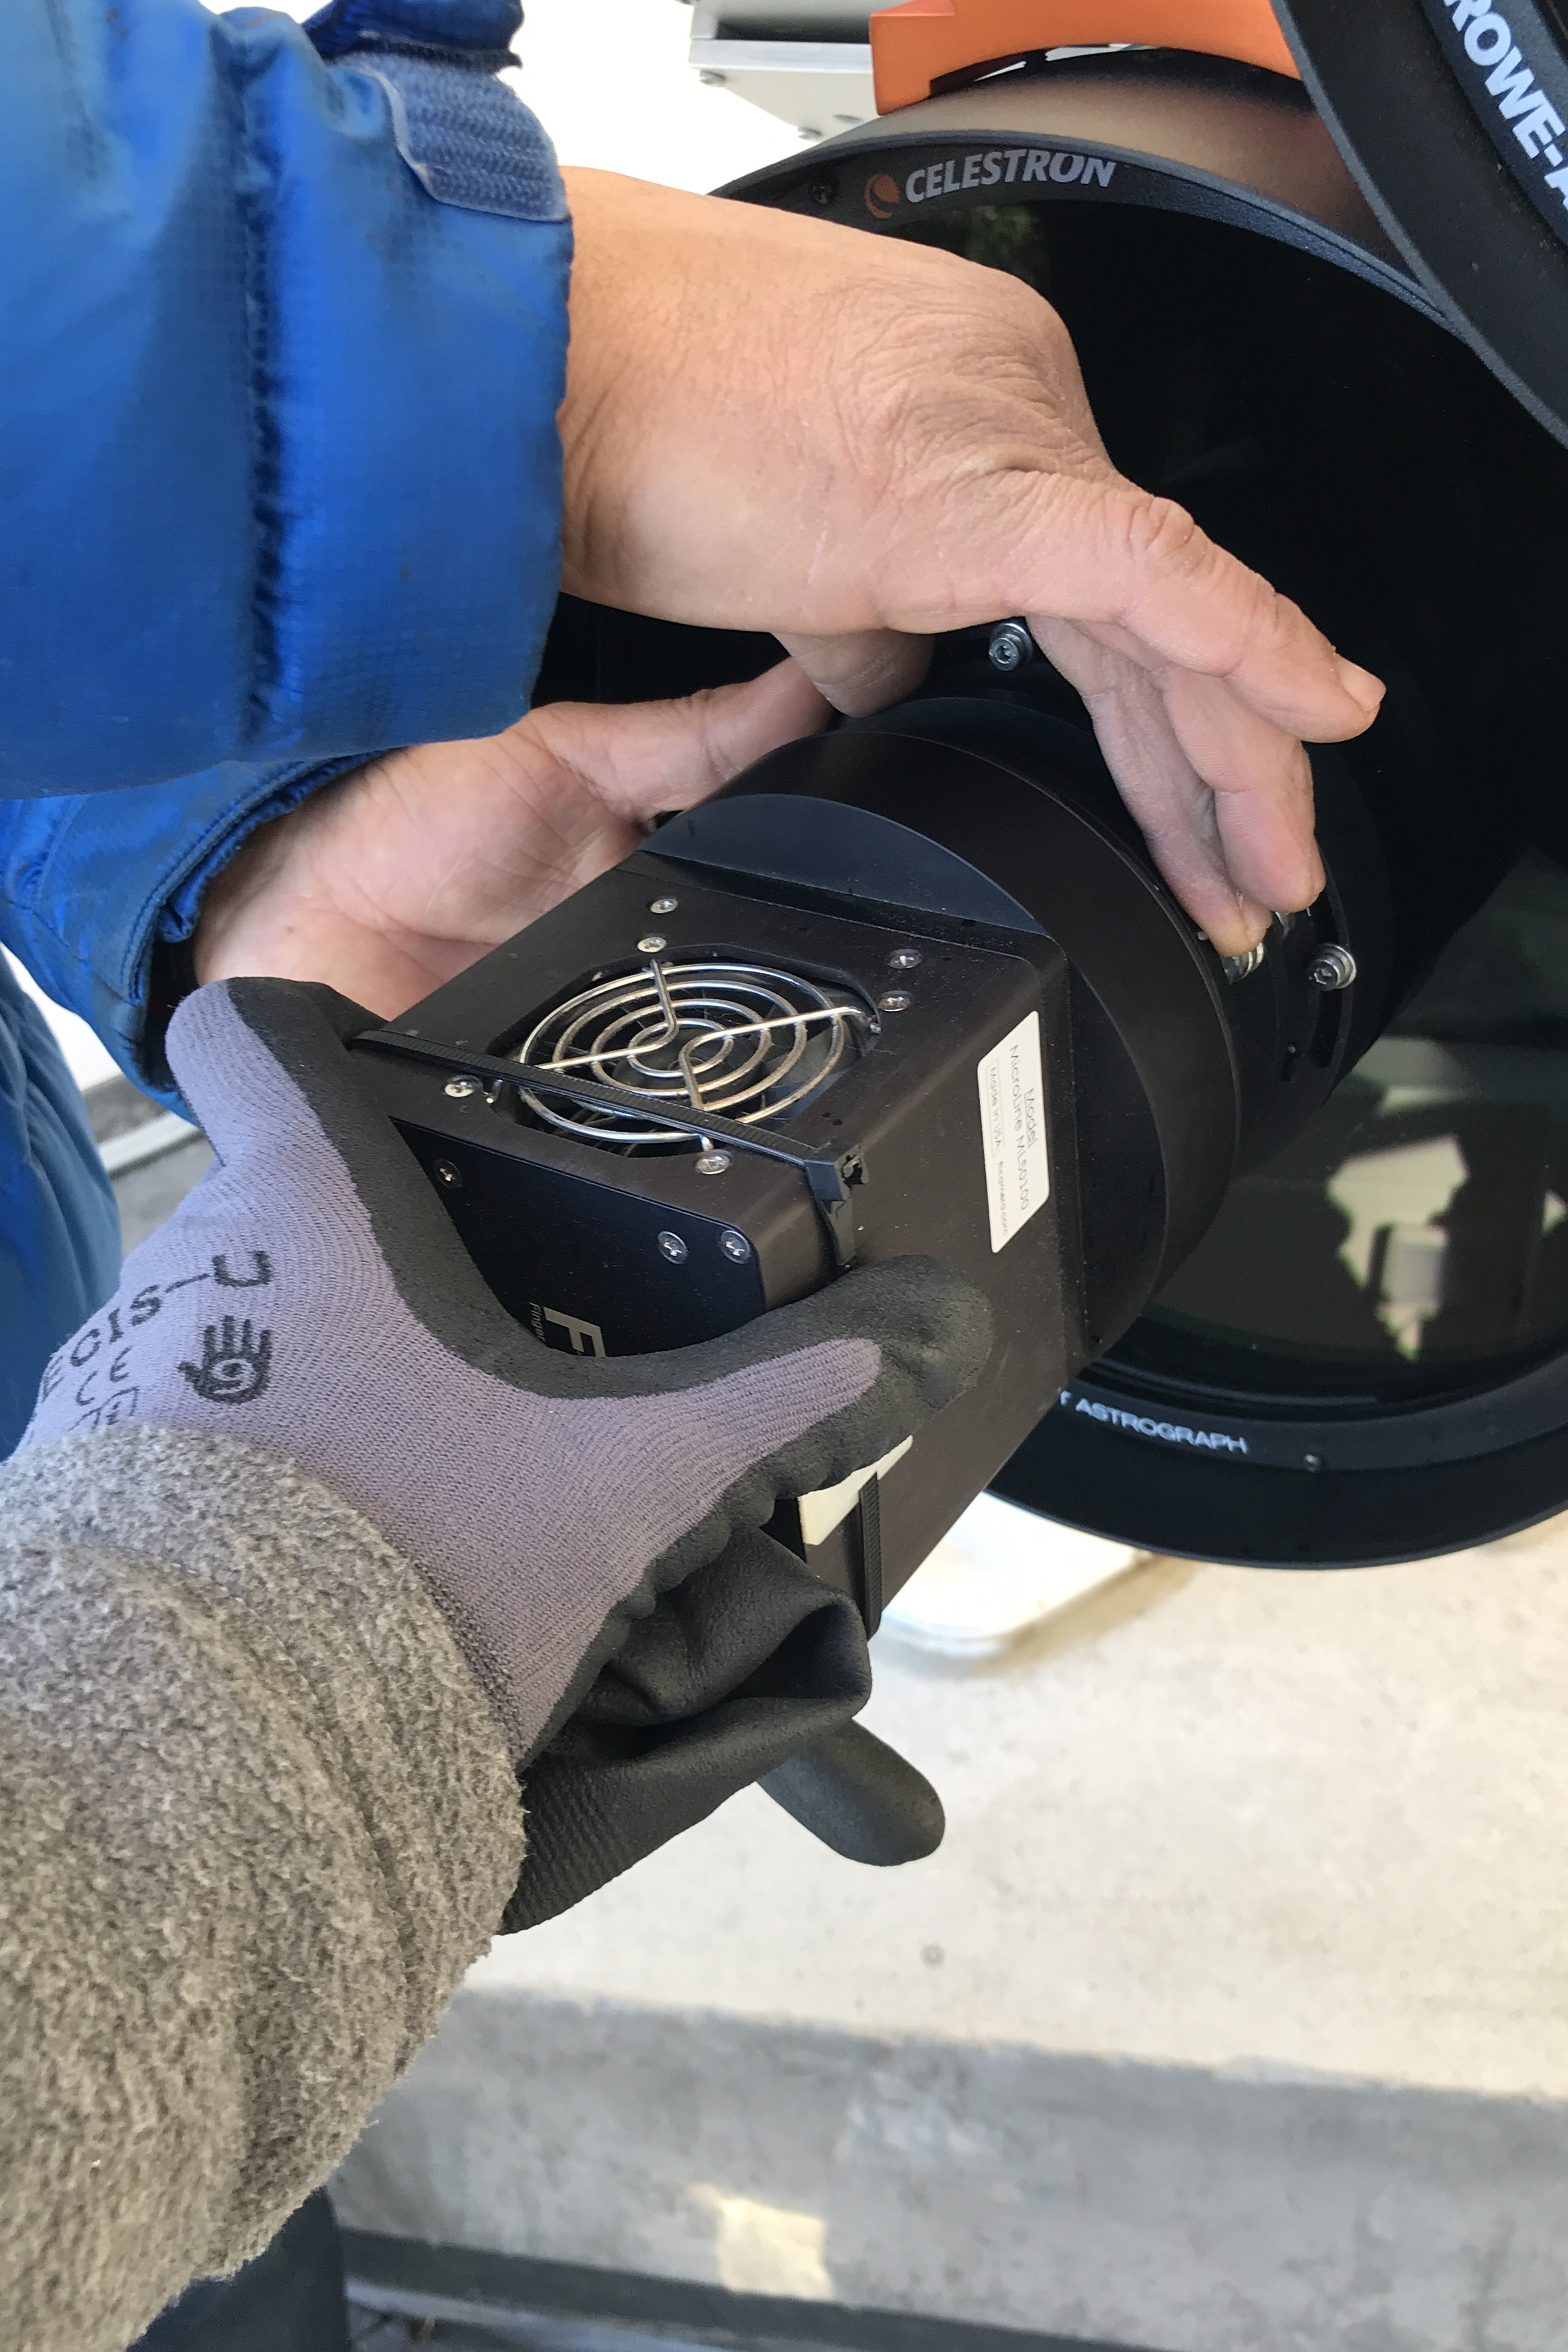
\includegraphics[height=0.7\linewidth]{figures/instrument-ddoti-removing-detector.jpg}
\end{center}
\caption{Removing the detector. One person should support the adapter against rotation while the other person unscrews the detector.}
\label{figure:instrument-ddoti-removing-detector}
\end{figure*}

\item While one person holds the tip tilt adapter to prevent it from placing a torque on the mounting ring, the other should gently unscrew the detector. See Figure~\ref{figure:instrument-ddoti-removing-detector}.

\begin{figure*}
\begin{center}
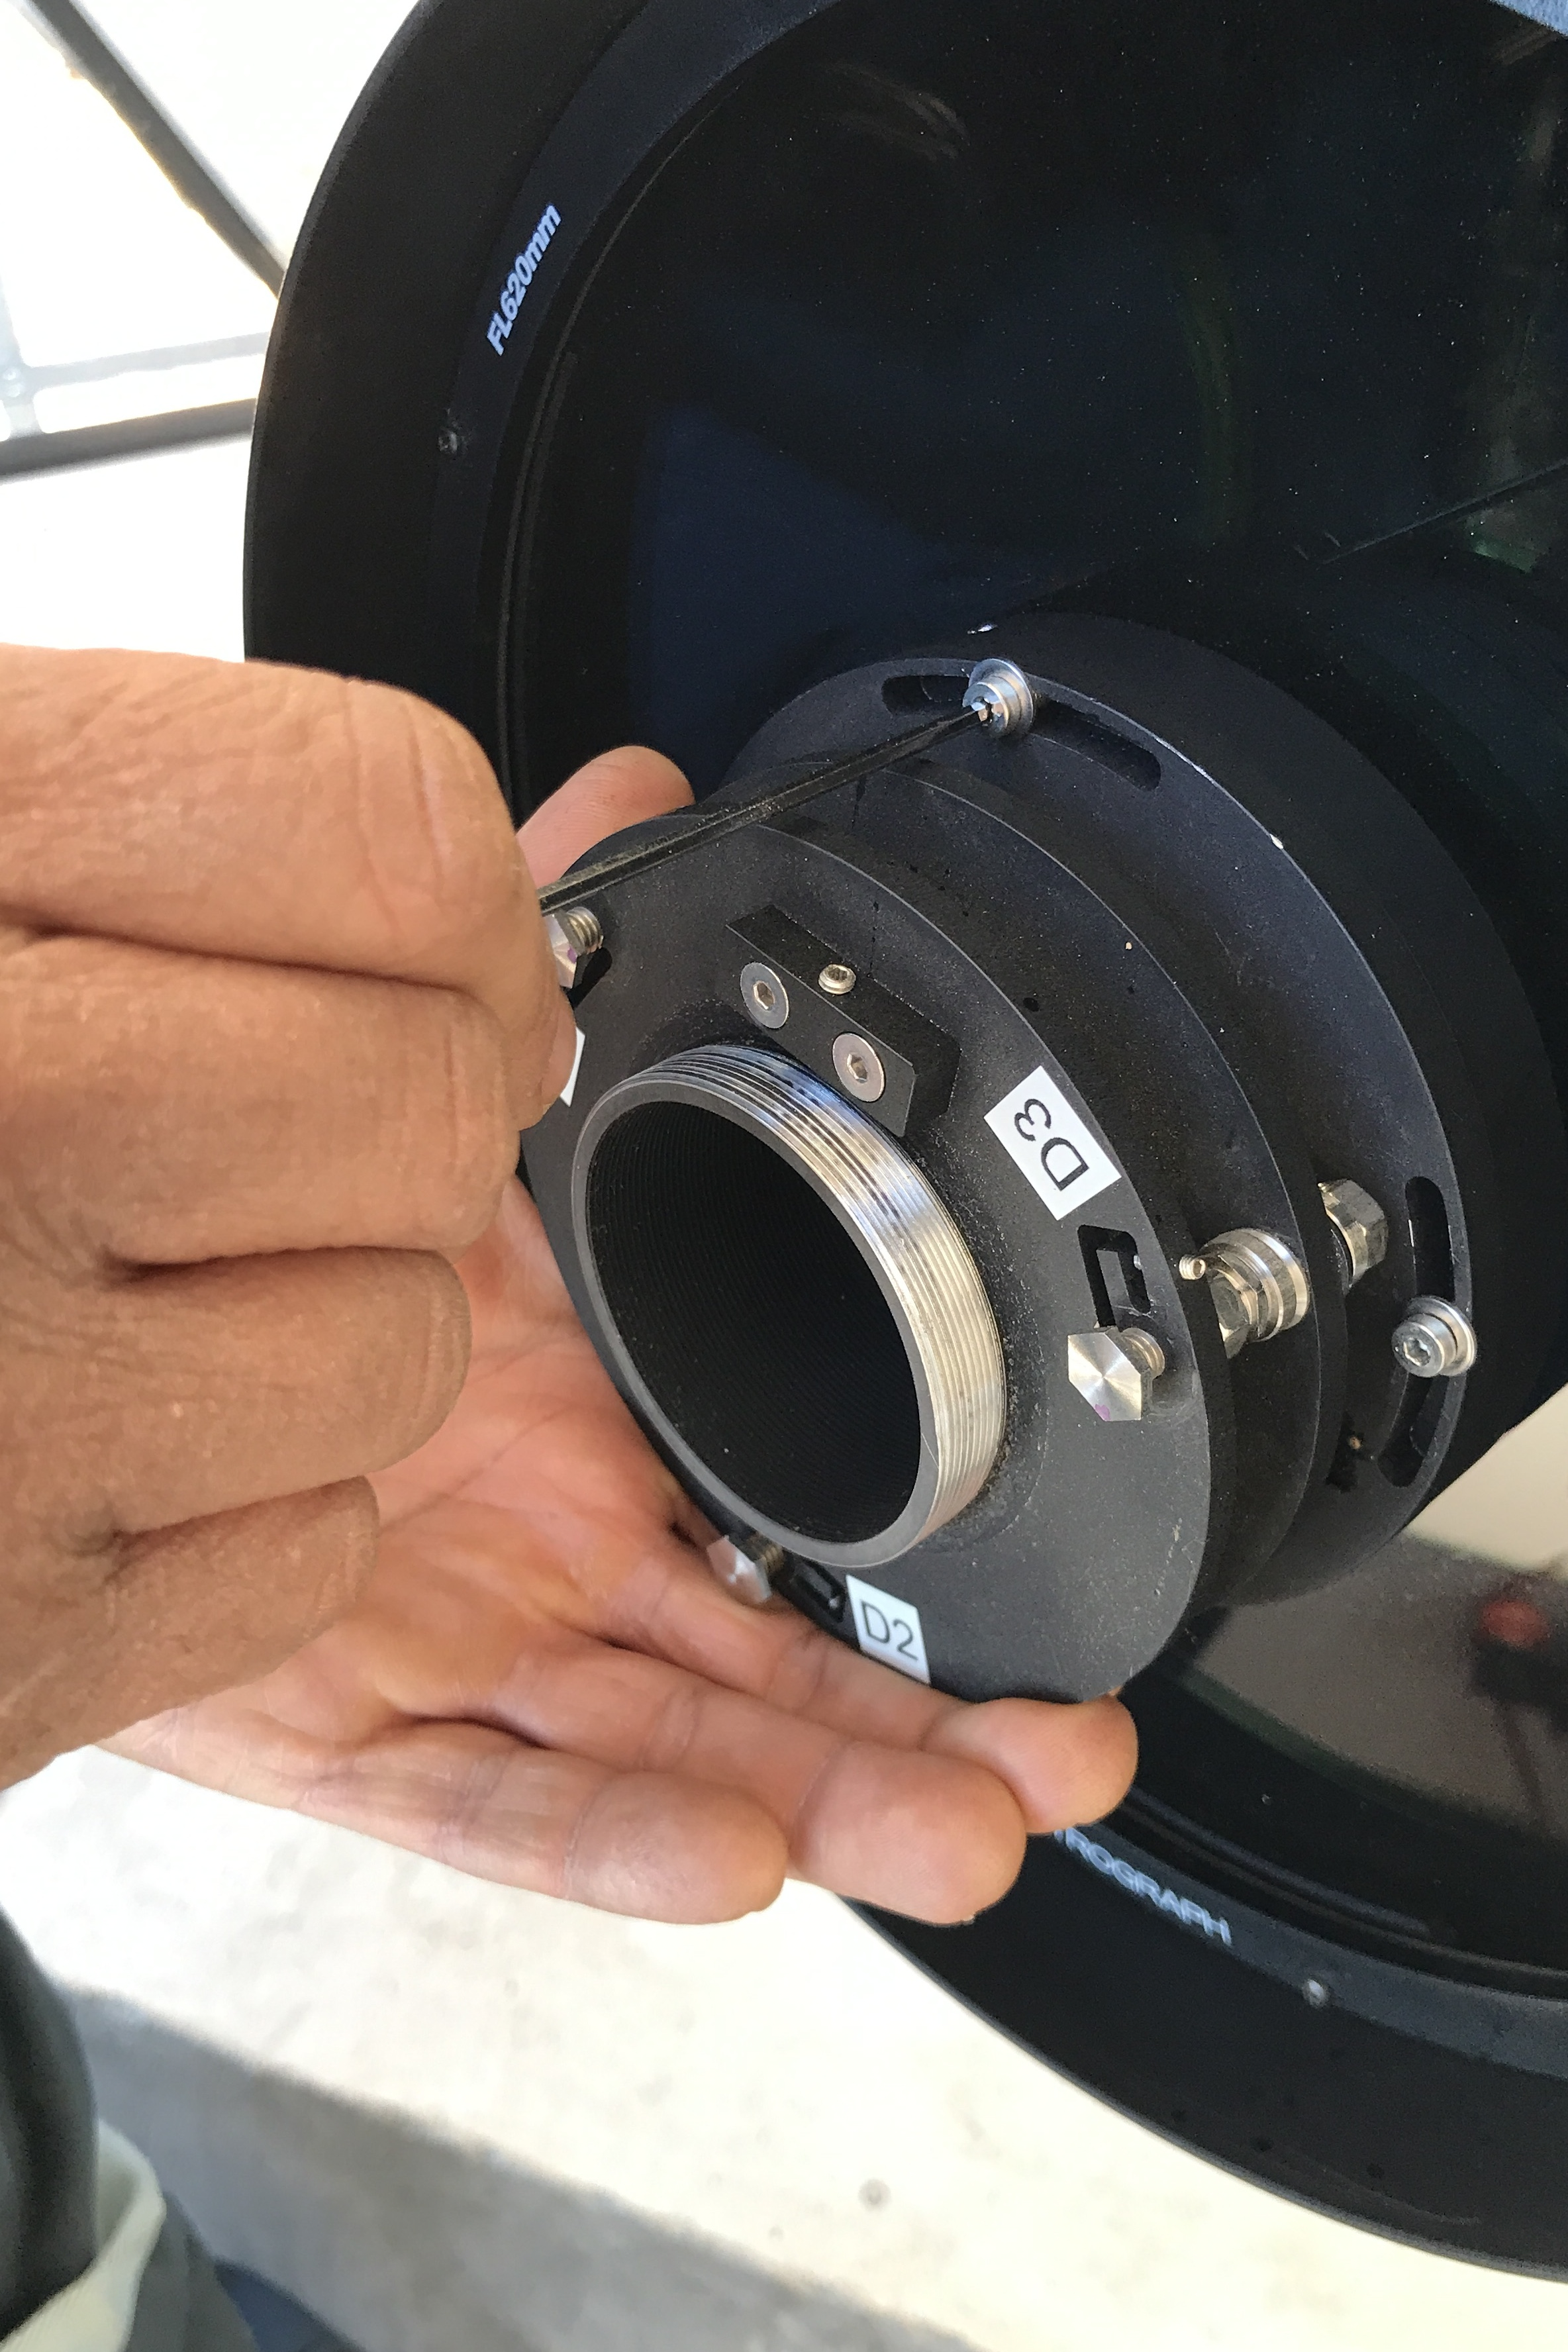
\includegraphics[height=0.7\linewidth]{figures/instrument-ddoti-removing-adapter.jpg}
\end{center}
\caption{Removing the adapter. Support the adapter with one hand to avoid placing a torque on the mounting ring.}
\label{figure:instrument-ddoti-removing-adapter}
\end{figure*}

\item Using a 2.5 mm hex key, gently slacken the screws that hold the adapter to the mounting ring. Support the adapter to prevent it from placing a torque on the mounting ring. See Figure~\ref{figure:instrument-ddoti-removing-adapter}.

\begin{figure*}
\begin{center}
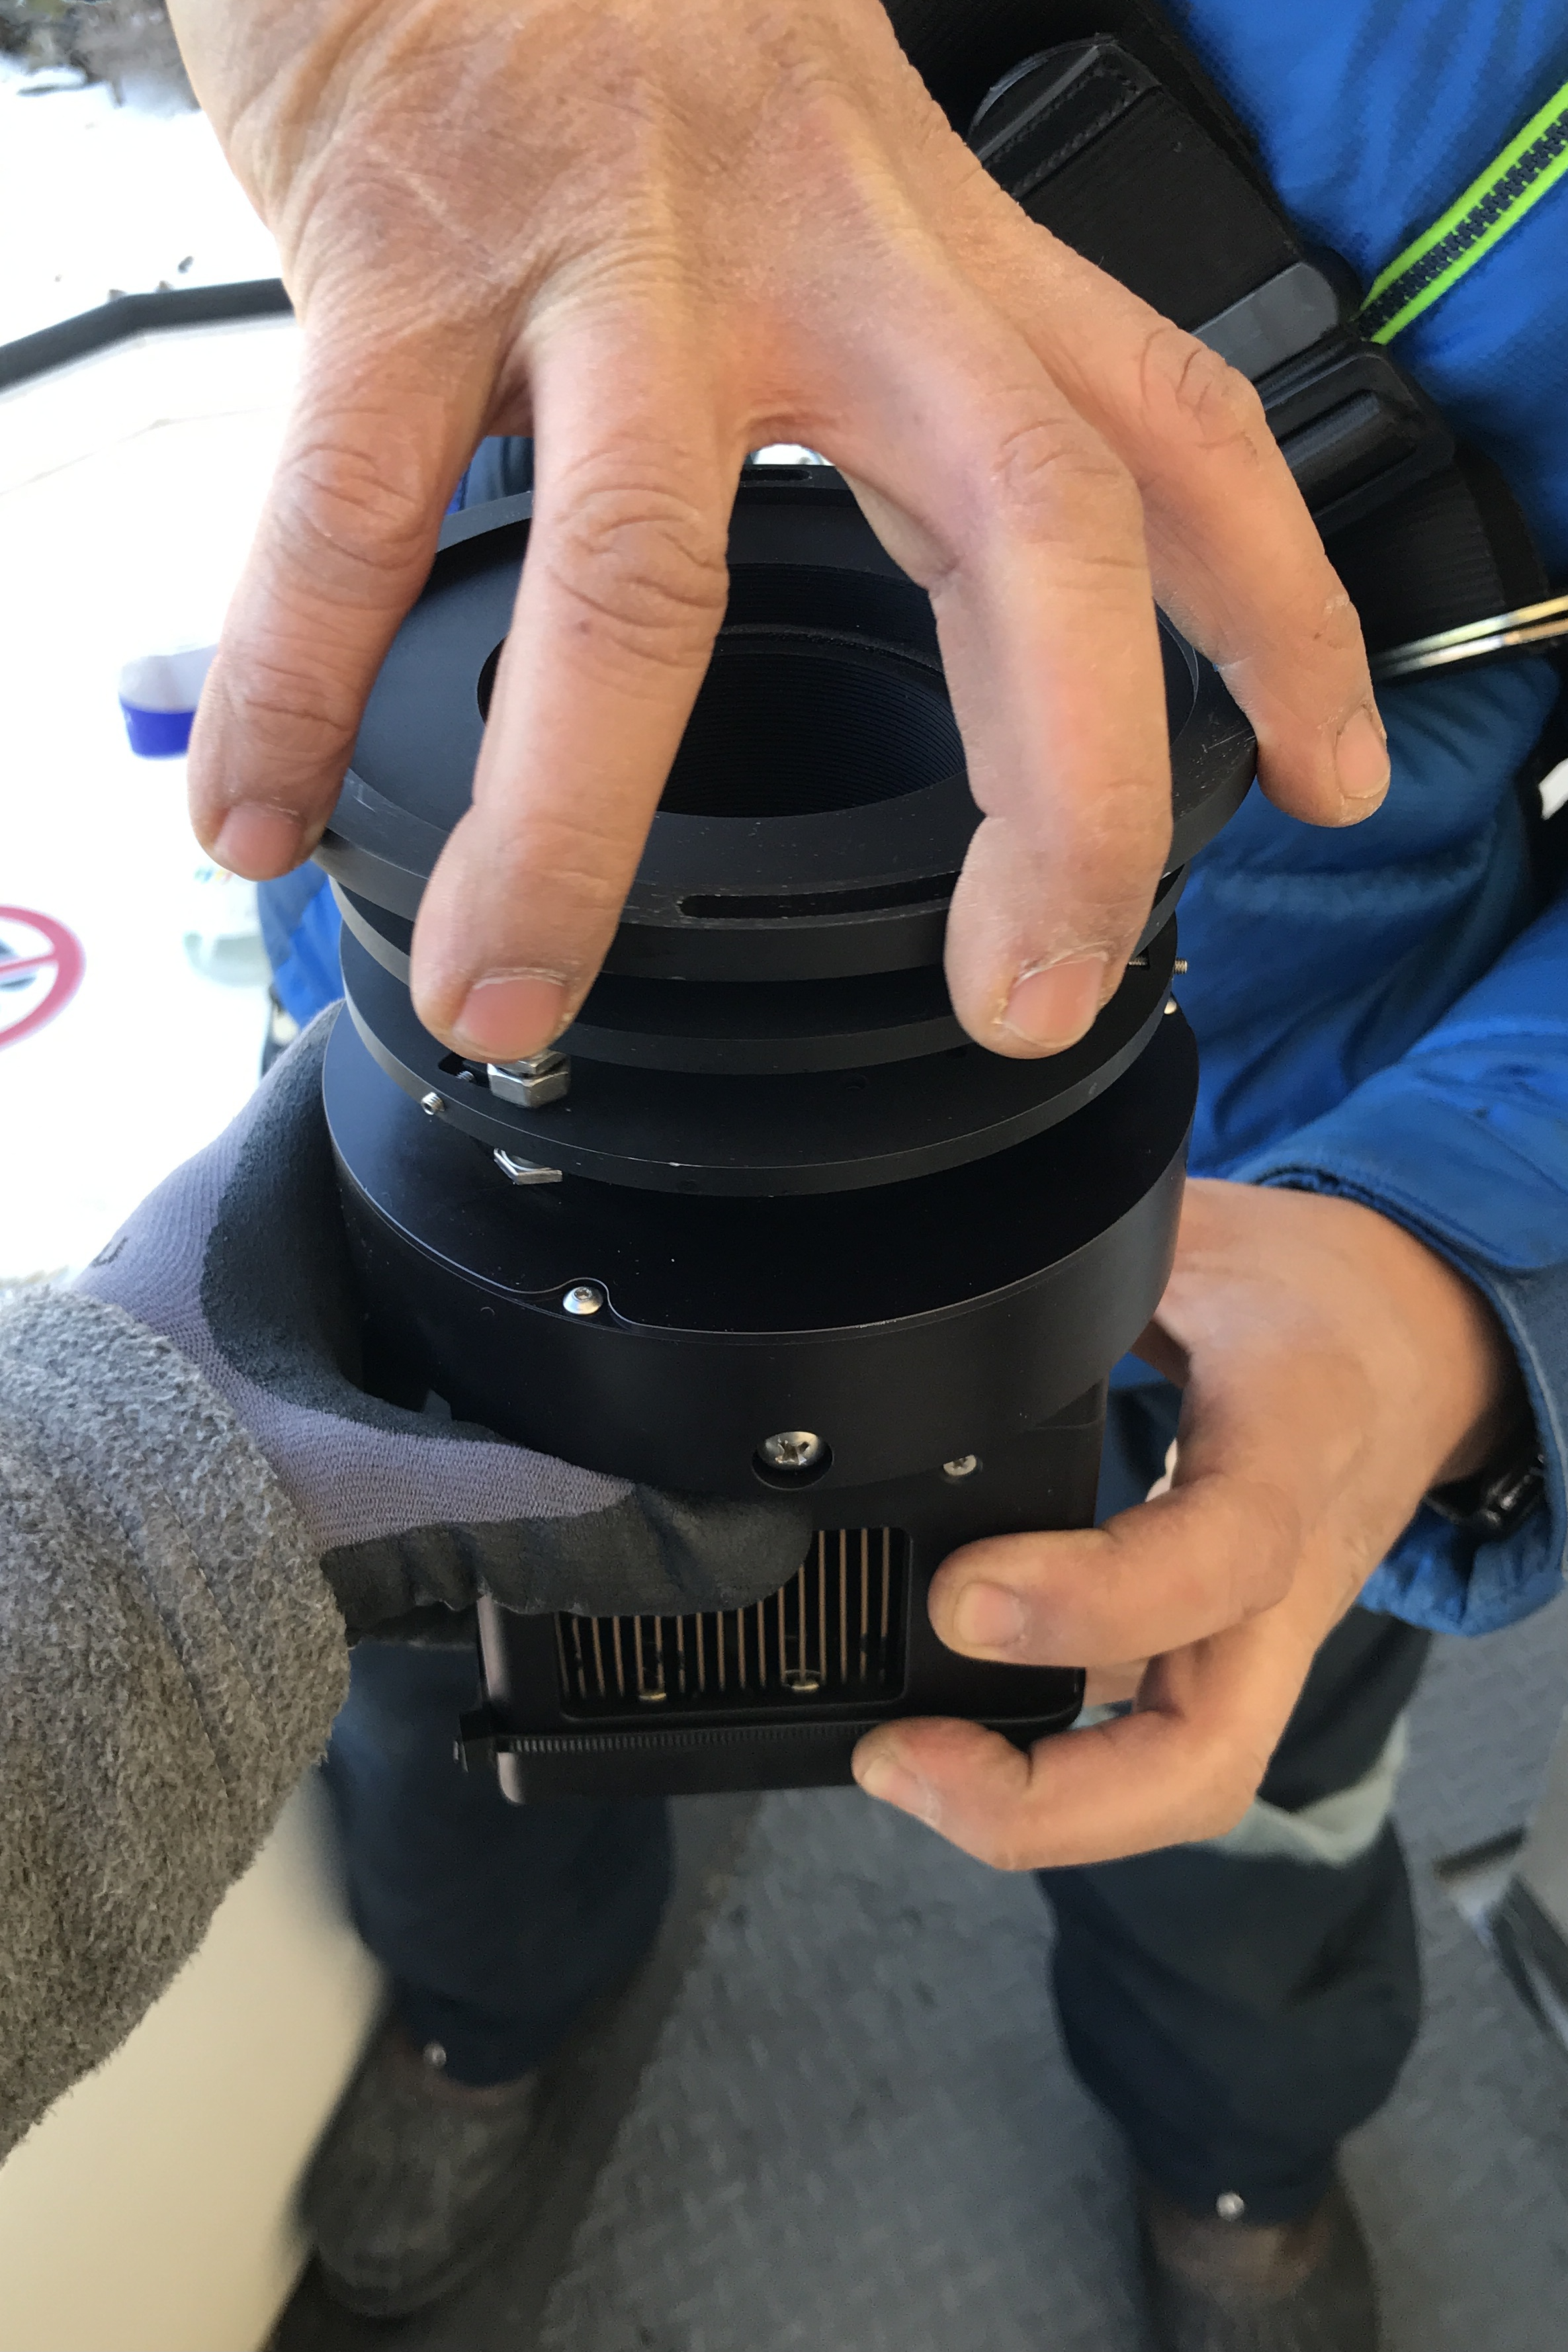
\includegraphics[height=0.7\linewidth]{figures/instrument-ddoti-attaching-detector.jpg}
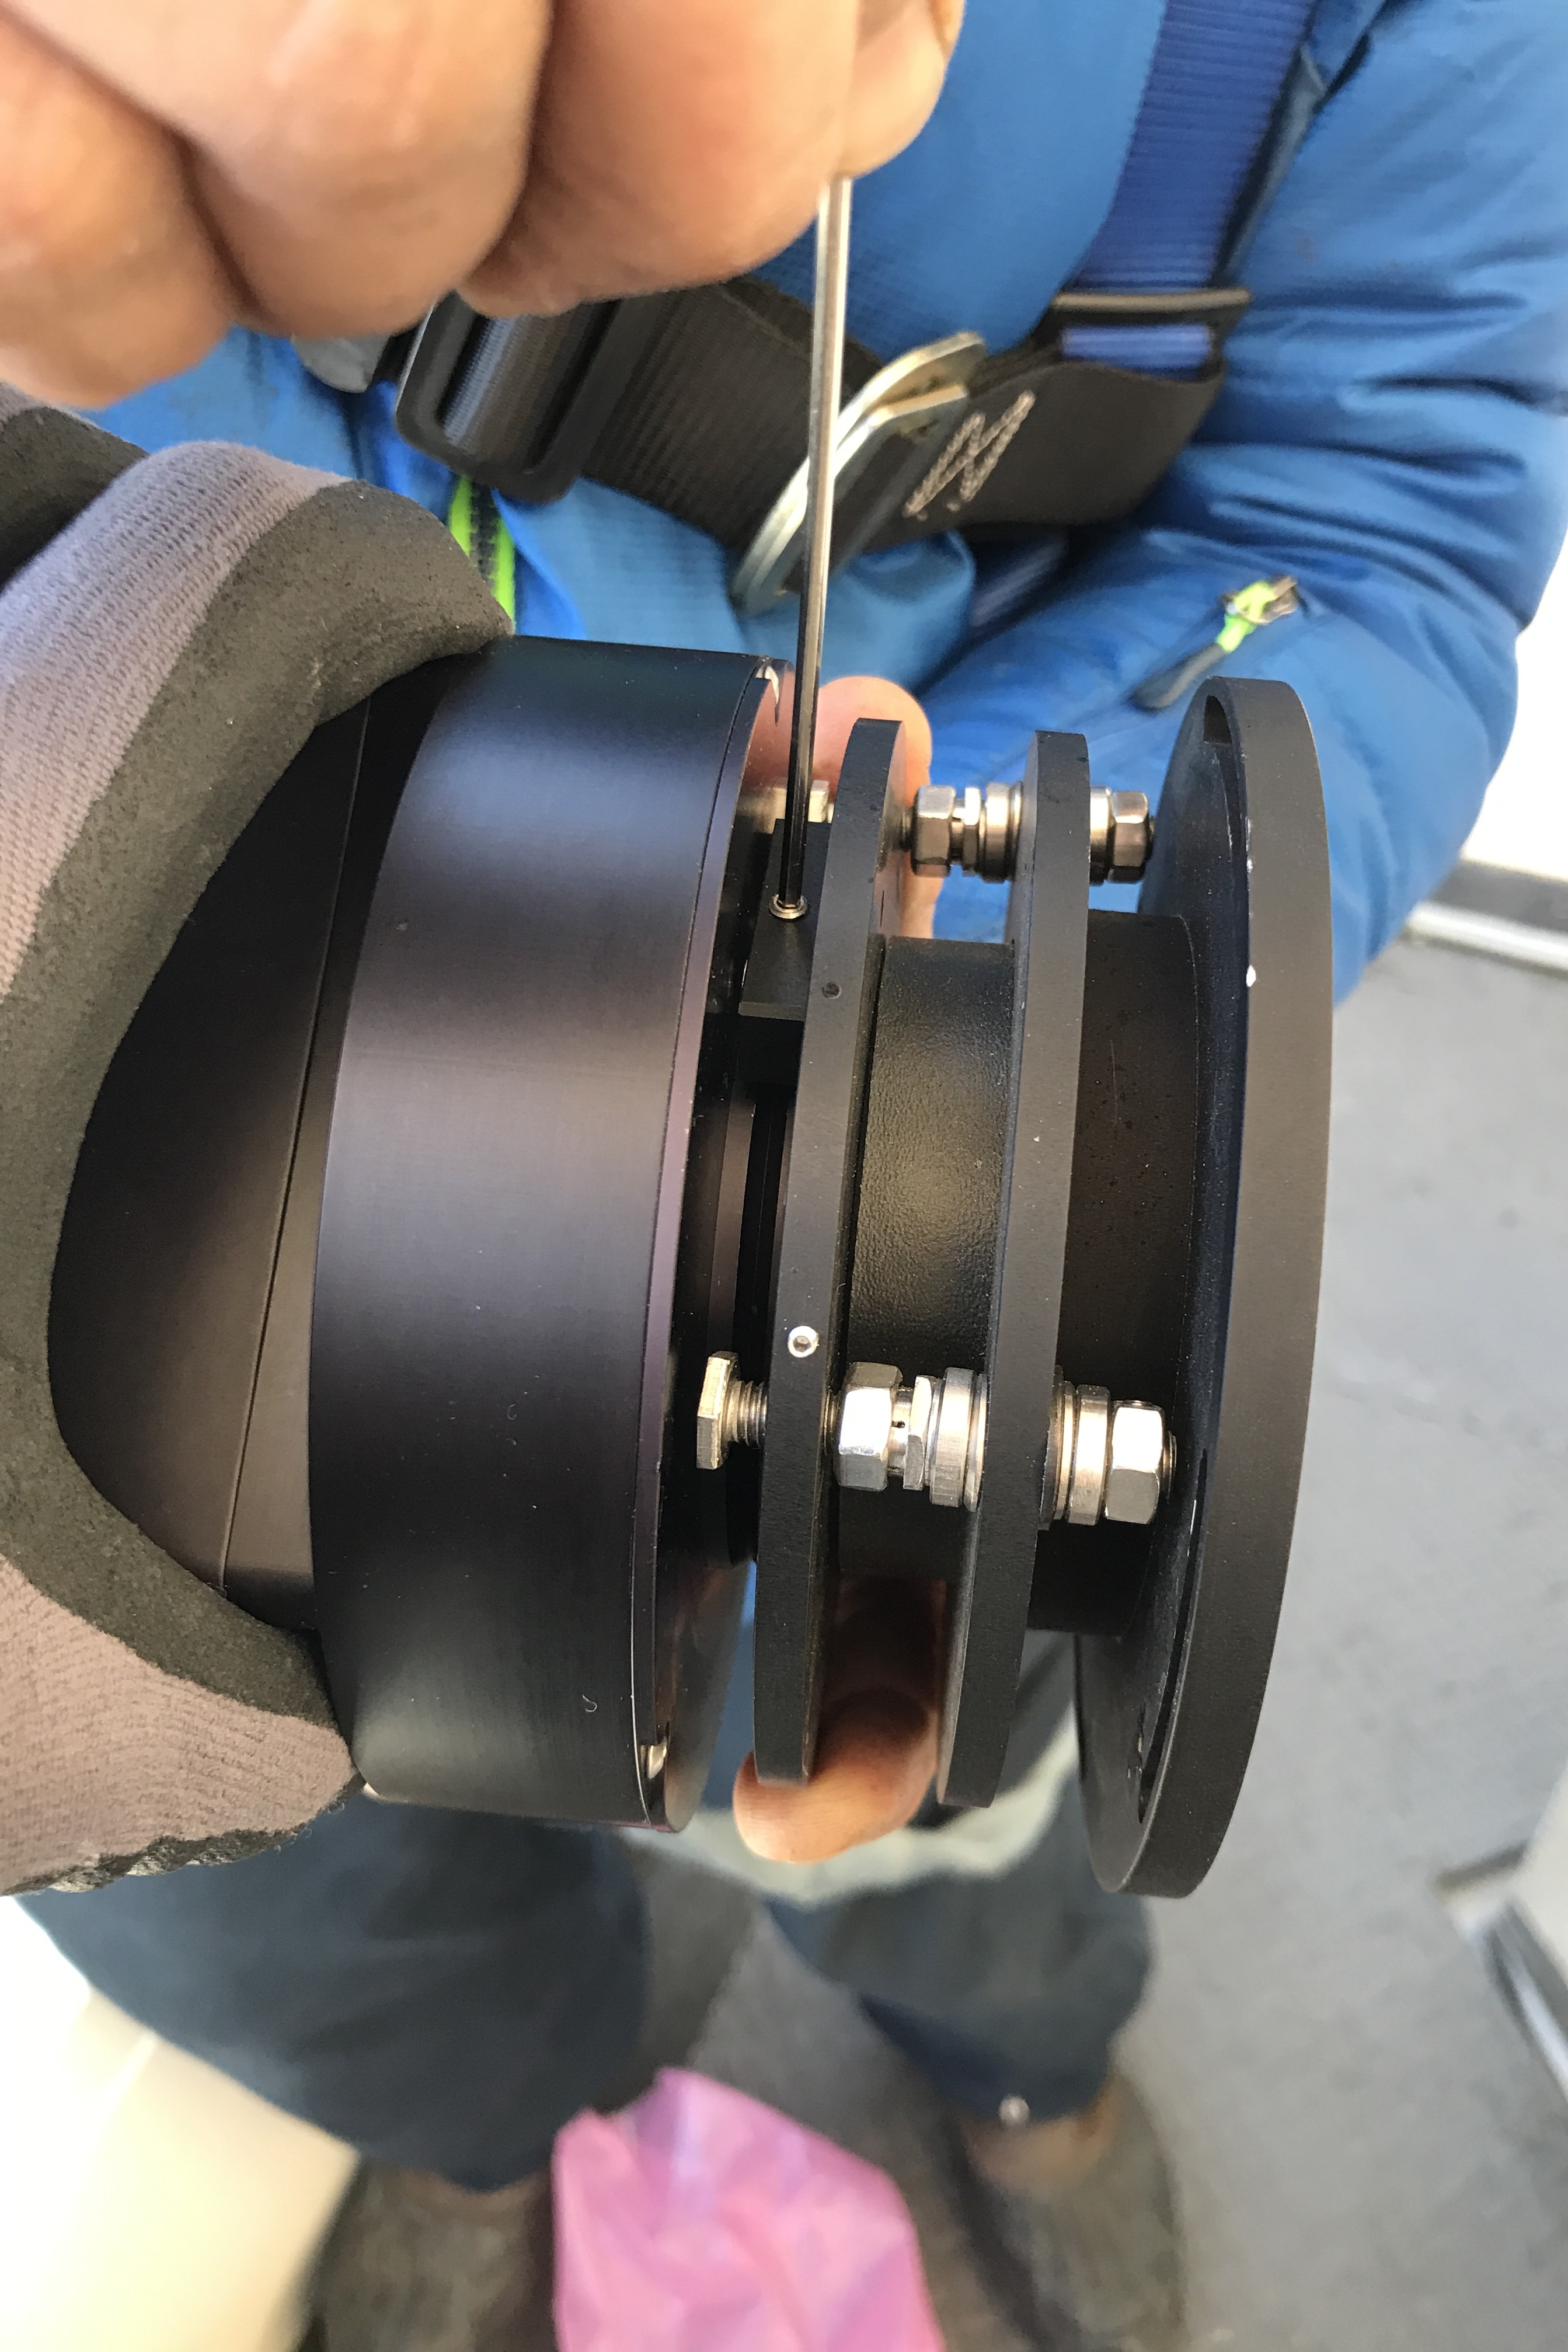
\includegraphics[height=0.7\linewidth]{figures/instrument-ddoti-tightening-grub-screw.jpg}
\end{center}
\caption{Attaching the new detector to the adapter.}
\label{figure:instrument-ddoti-attaching-detector}
\end{figure*}

\item Screw the new detector into the adapter and tighten the grub screw. See Figure~\ref{figure:instrument-ddoti-attaching-detector}.

\begin{figure*}
\begin{center}
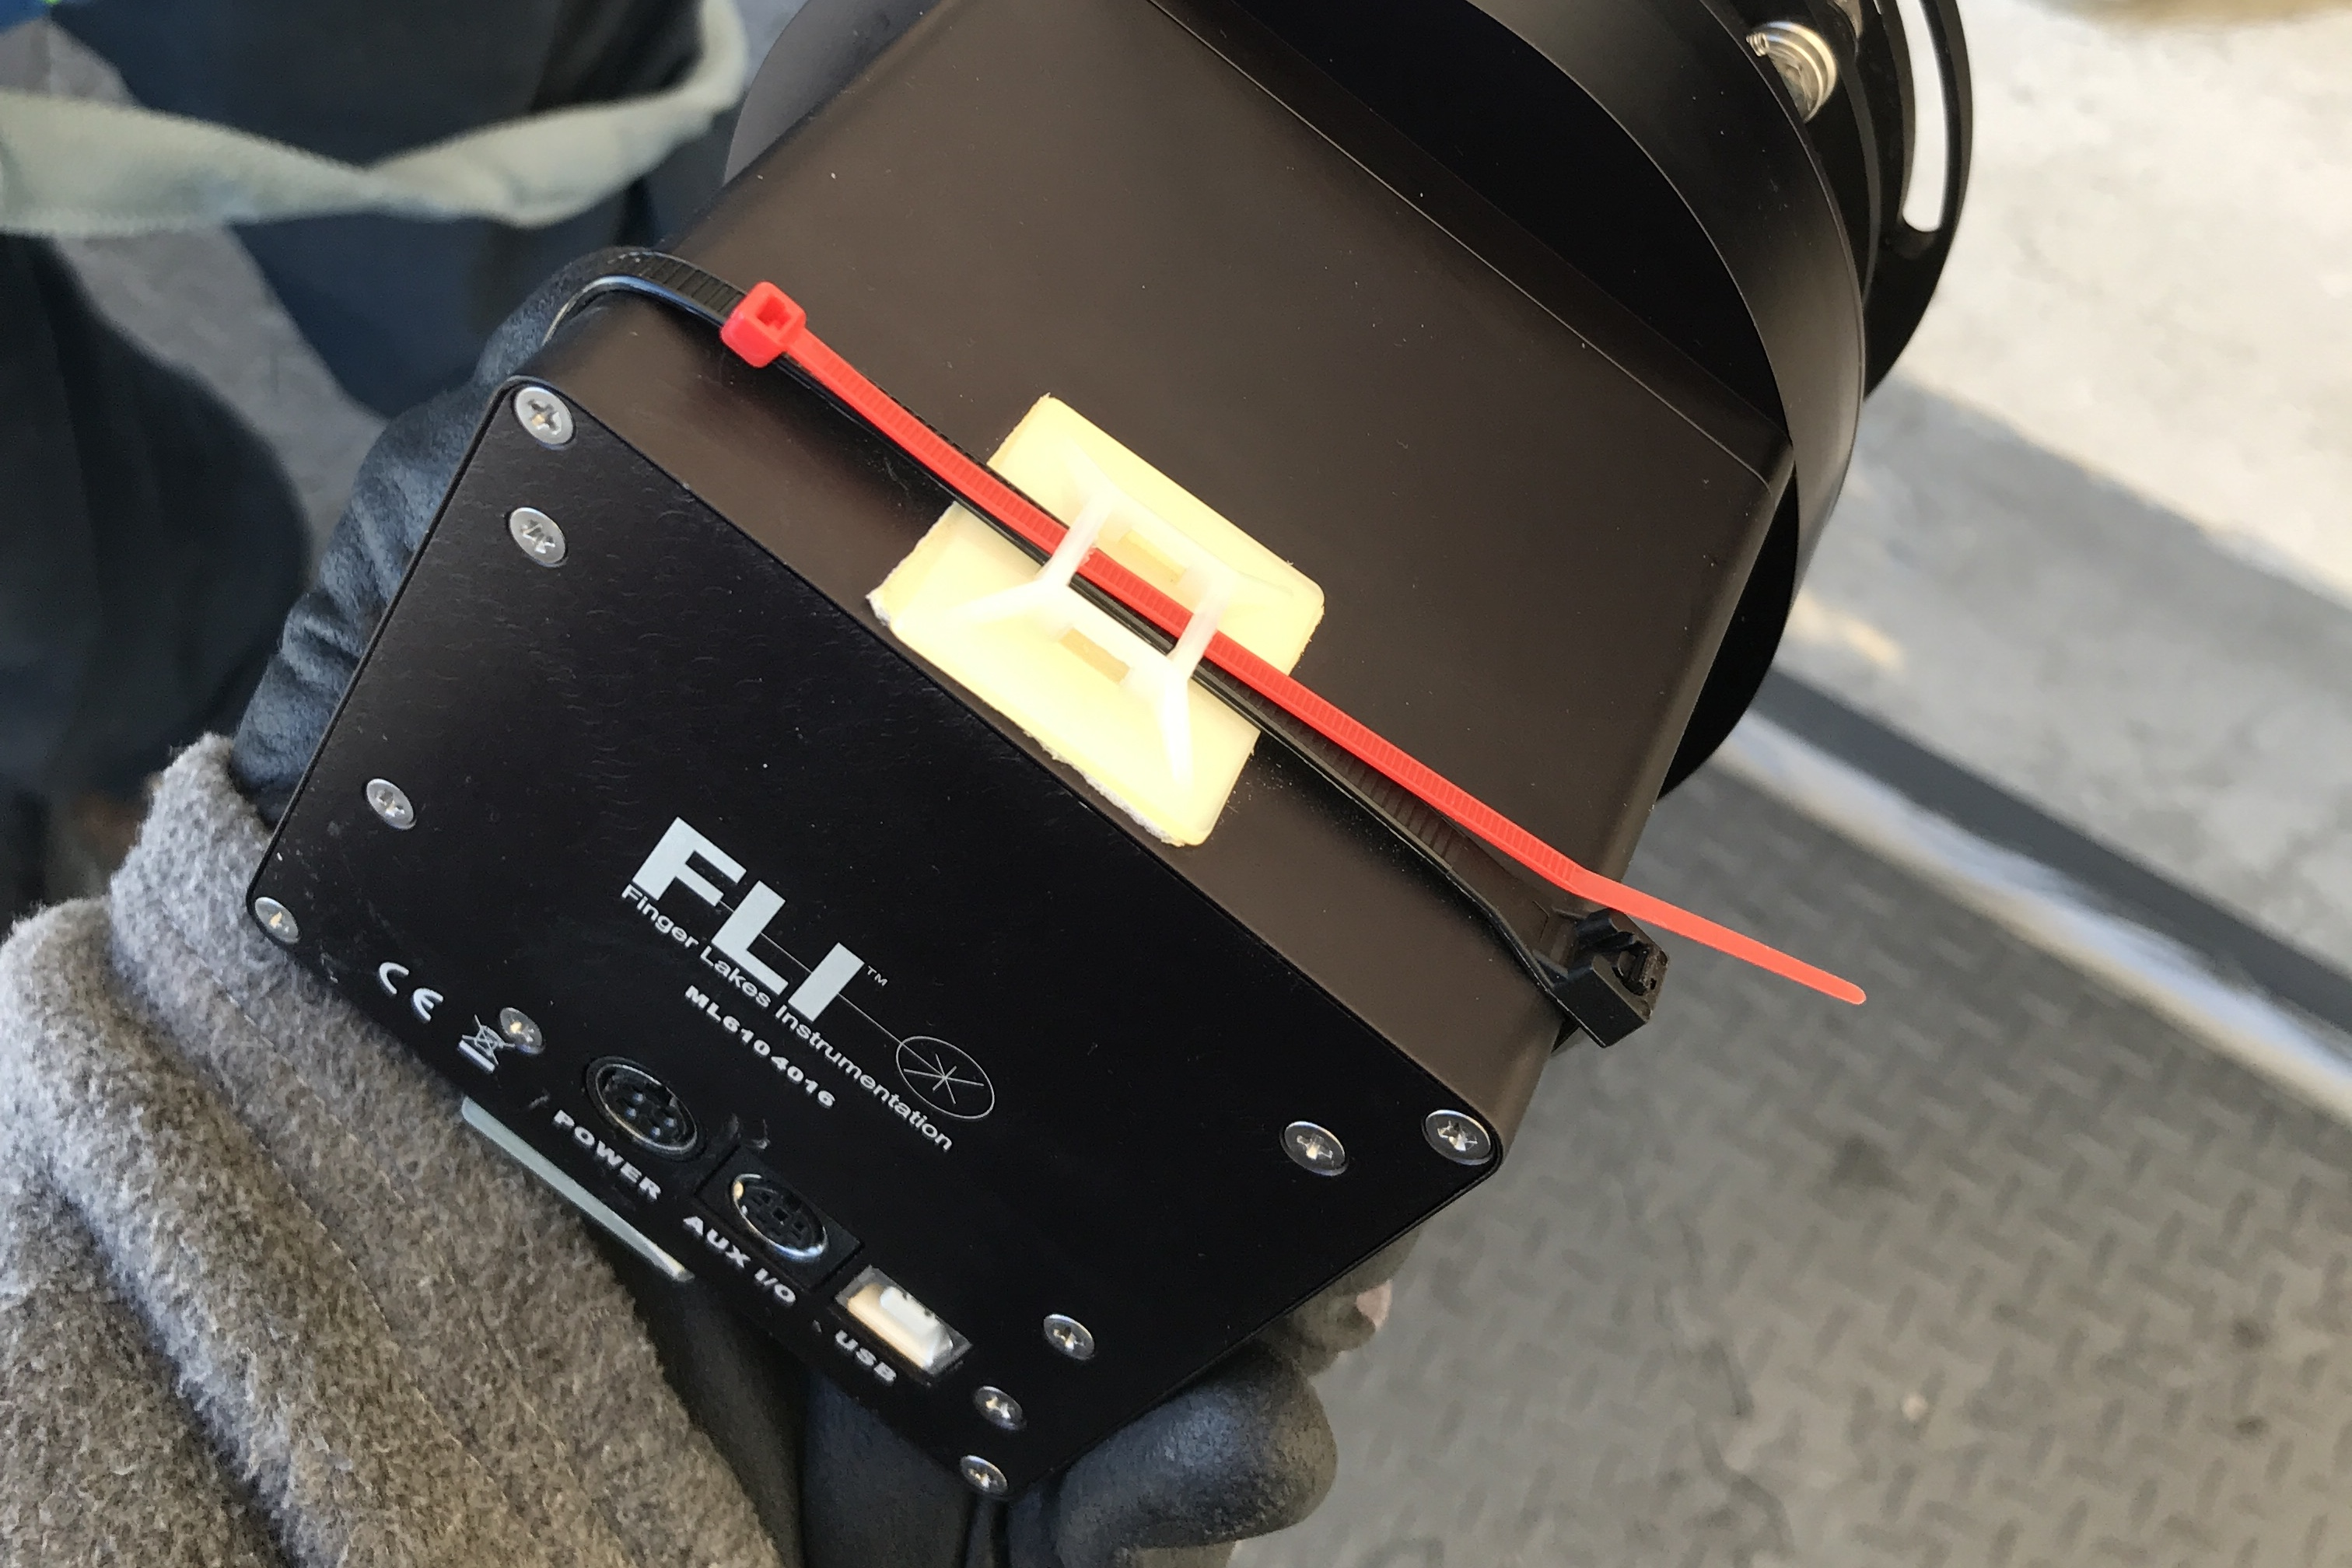
\includegraphics[width=0.7\linewidth]{figures/instrument-ddoti-attaching-cable-tie.jpg}
\end{center}
\caption{Attaching a cable tie to the detector prior to mounting it on the telescope.}
\label{figure:instrument-ddoti-attaching-cable-tie}
\end{figure*}

\item Thread a small cable tie through the appropriate base. It is important to do this before you attach the adapter to the mounting ring, to avoid placing a torque on the mounting ring. See Figure~\ref{figure:instrument-ddoti-attaching-cable-tie}.

\begin{figure*}
\begin{center}
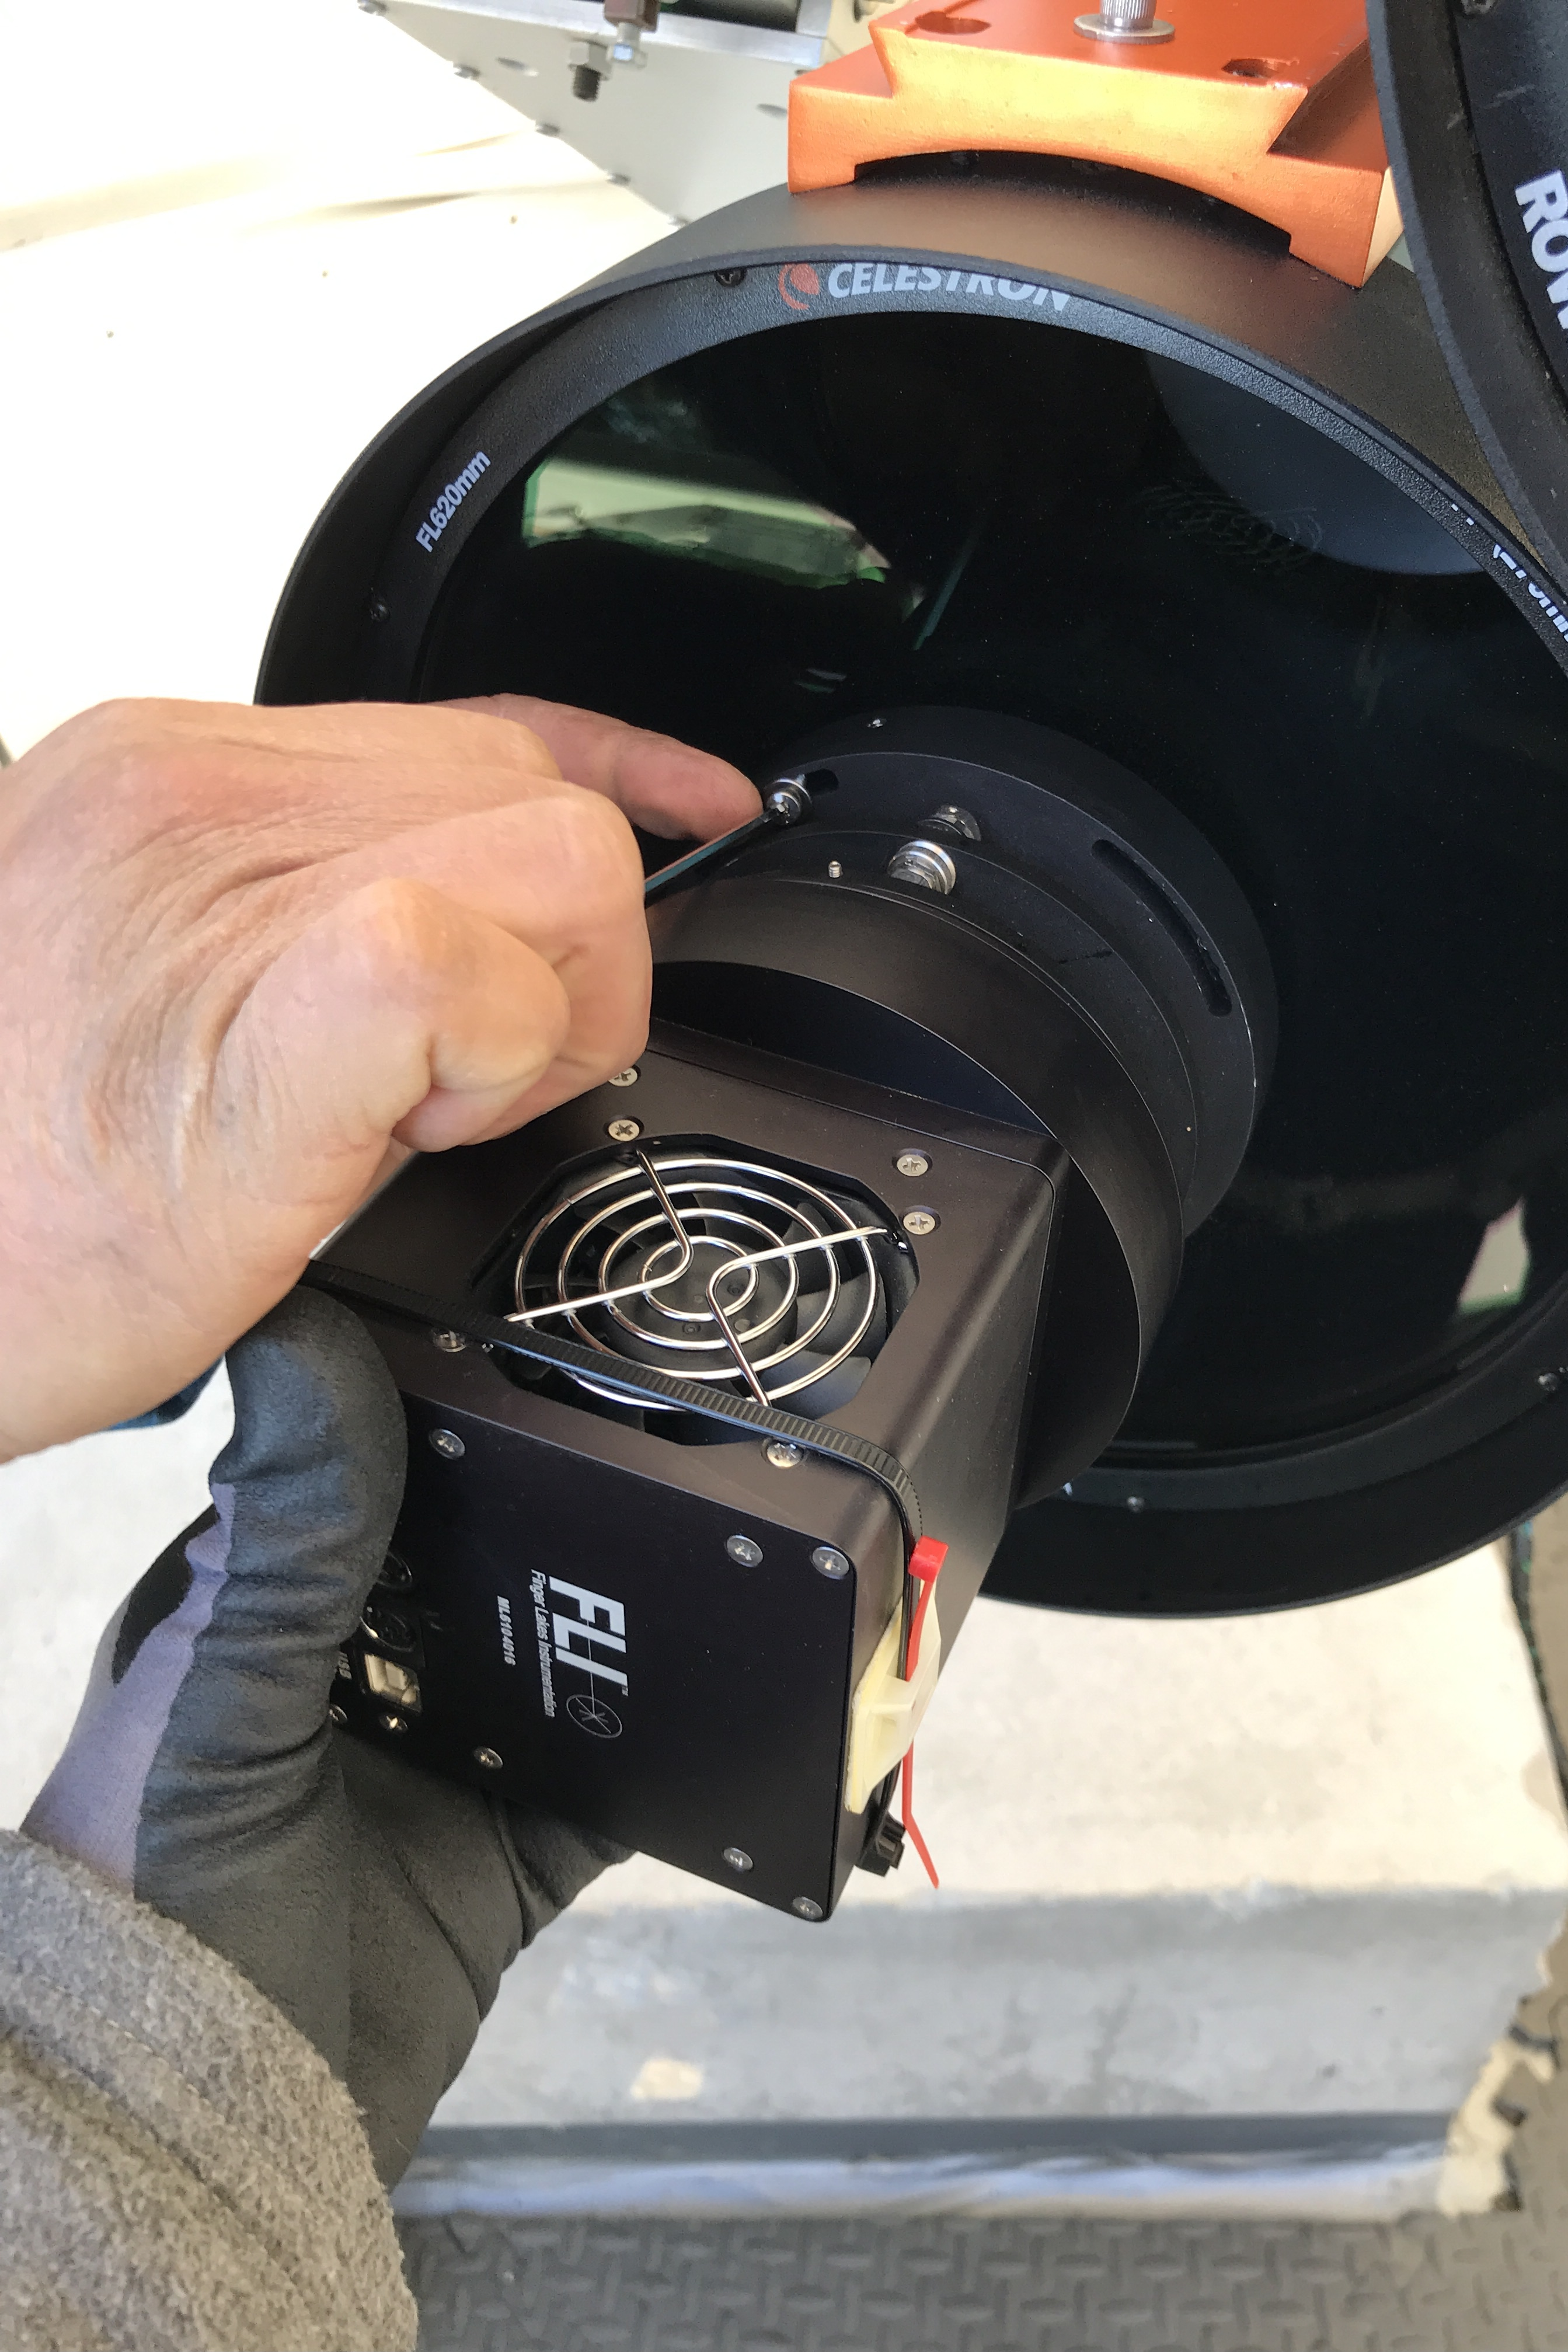
\includegraphics[height=0.7\linewidth]{figures/instrument-ddoti-attaching-adapter}
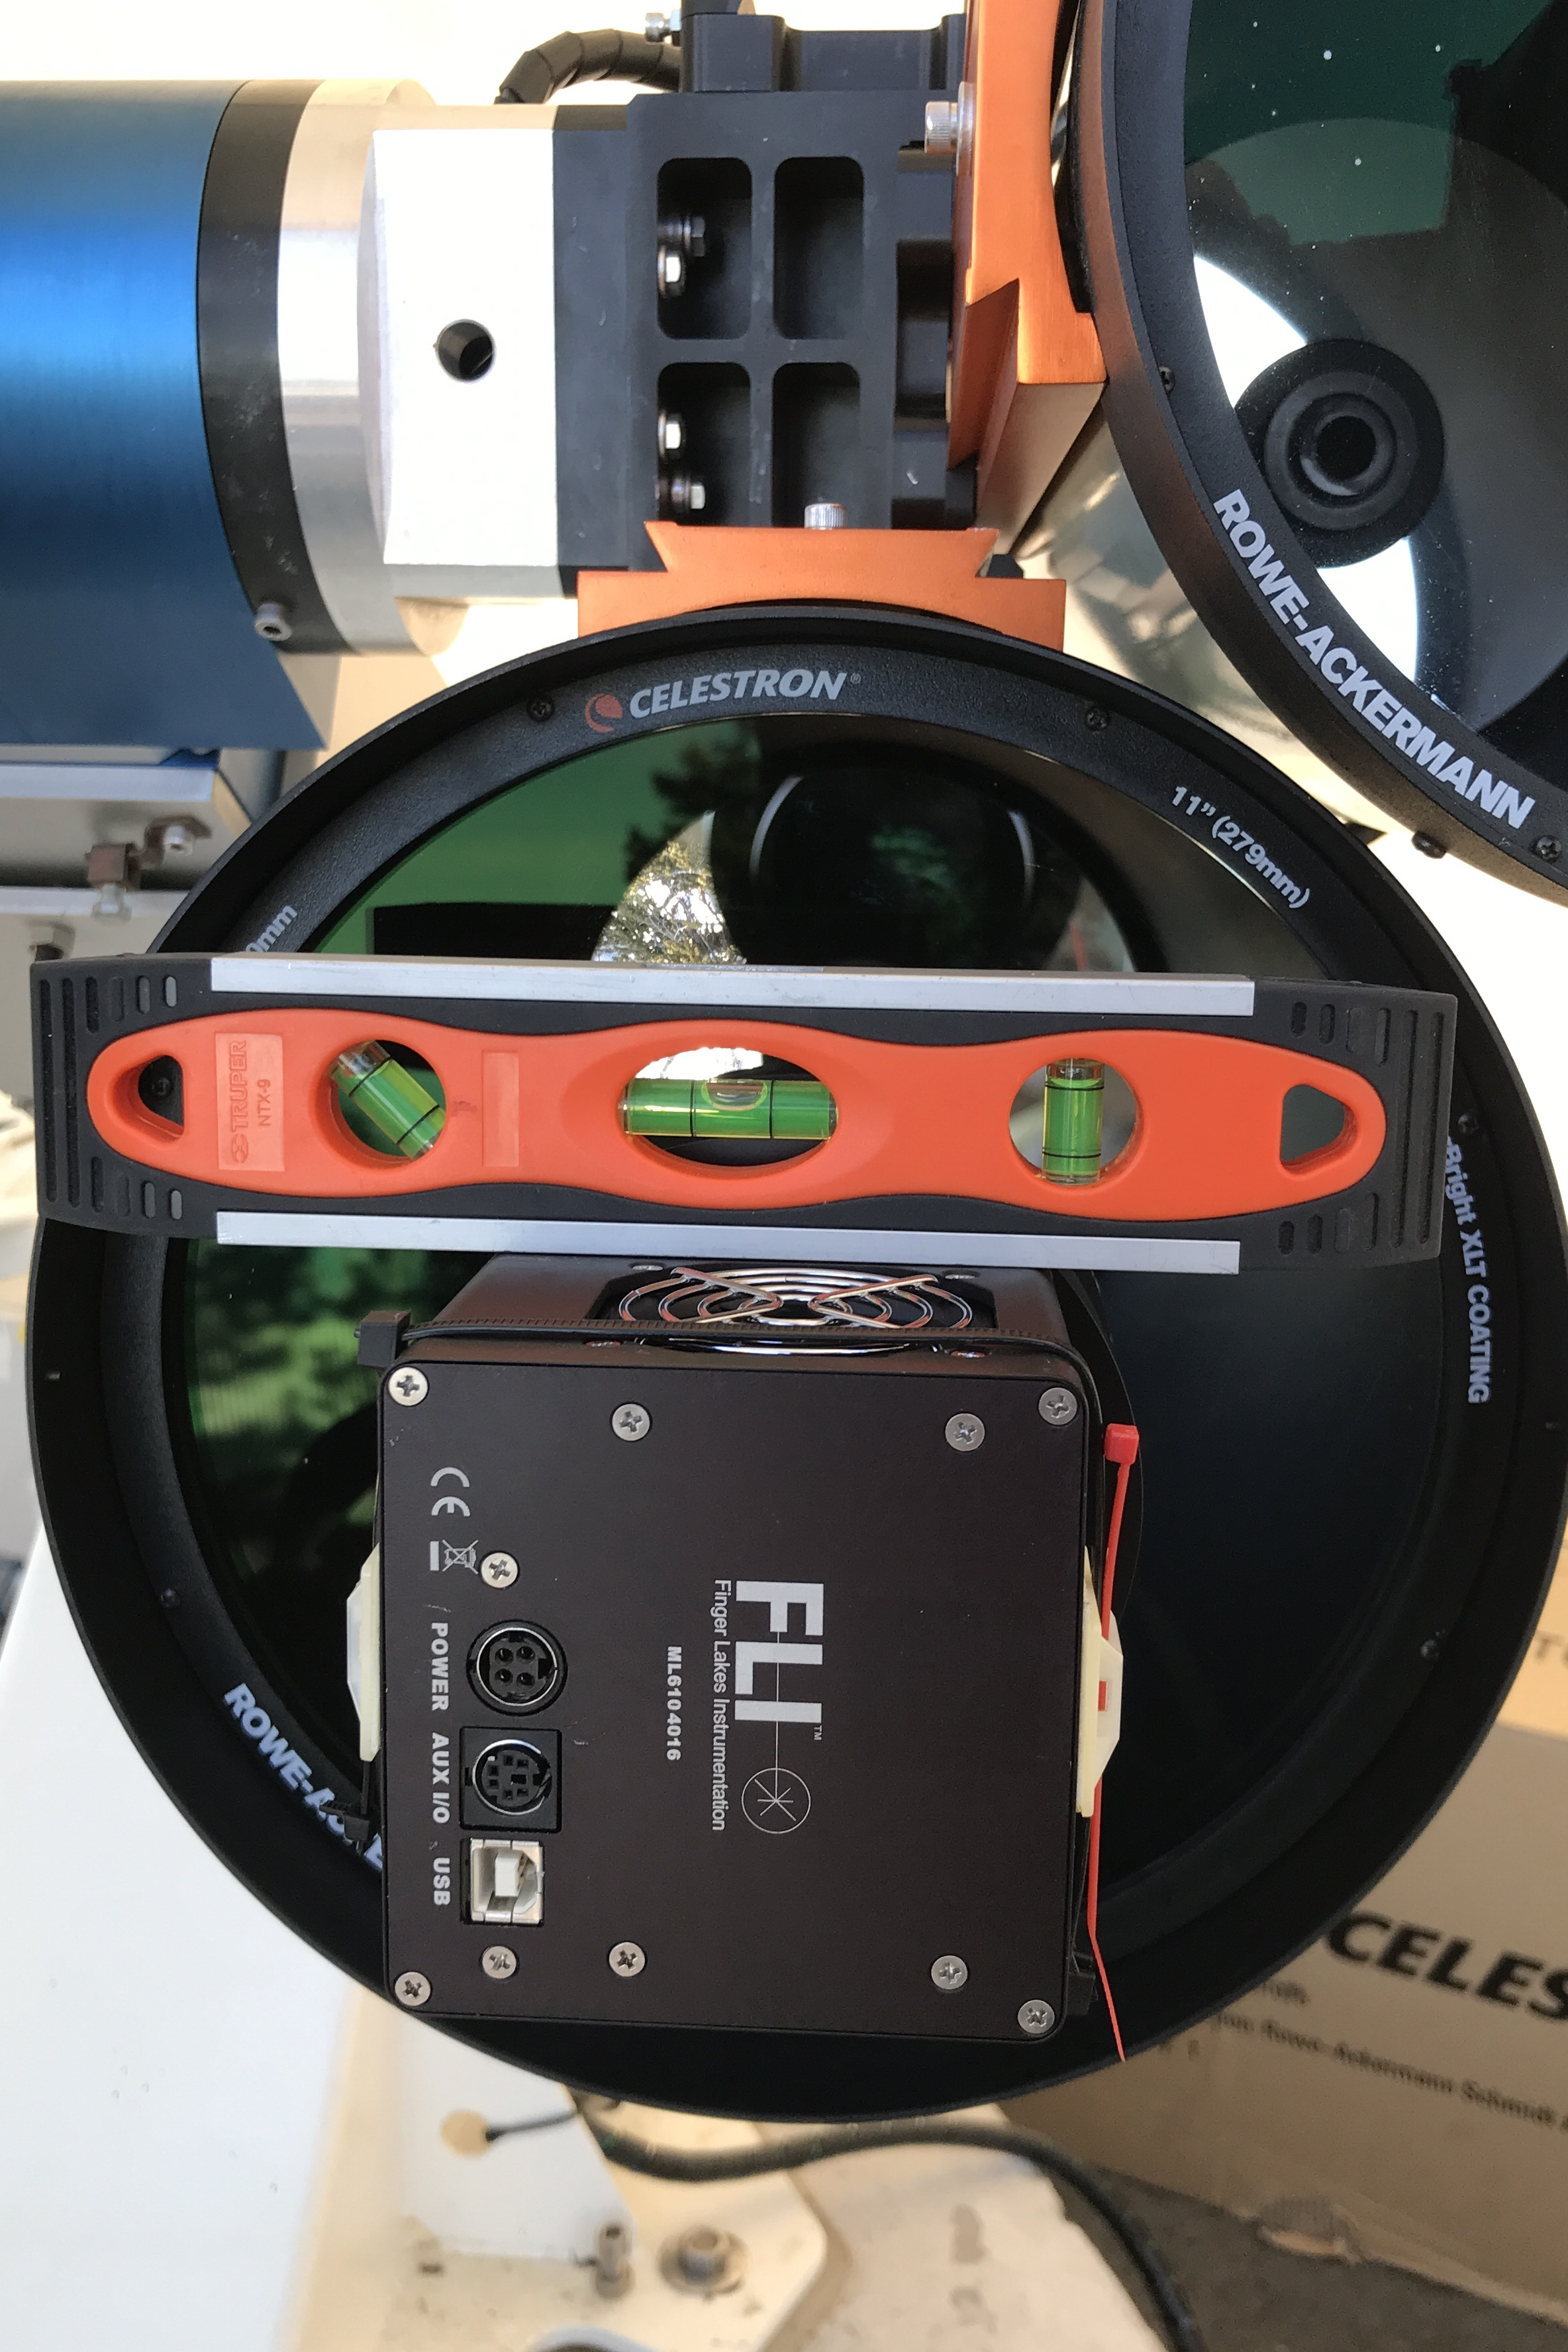
\includegraphics[height=0.7\linewidth]{figures/instrument-ddoti-detector-level}
\end{center}
\caption{Attaching the adapter to the mounting ring. Be careful to avoid placing a torque on the mounting ring.}
\label{figure:instrument-ddoti-attaching-adapter}
\end{figure*}

\item Attach the adapter to the mounting ring. All of the detectors have the same orientation, so you can use the others as guides. You can select the appropriate set of holes to give approximate alignment and then gently rotate the adapter in its slots for fine alignment. Use a level to guide you.
Make sure the hex screws are adequately lose before turning the adapter, to avoid placing a torque on the mounting ring. See Figure~\ref{figure:instrument-ddoti-attaching-adapter}.

\item Attach the cables to the detector and secure them with the cable tie. Support the detector to prevent it from placing a torque on the mounting ring.

\item Communicate with the DDOTI team who will configure the new detector in the control system, restart the software, and verify that the detector is integrated correctly.

\item Descend from the platform.

\item Close the enclosure. If the red error button is lit or flashing, press it to clear the error. (Often you will activate the safety strip when entering or leaving the enclosure.) Press and hold the “CLOSE” button until the green light goes off.

\item 
Move the enclosure controller mode selector switch to “REMOTE”.

\item
Replace all tools and equipment in their correct places.
\end{enumerate}

\section{Calibration Data}

\subsection{Biases and Darks}

\subsection{Flats}

\subsection{Gain and Read Noise}

The control system does not automatically take data for calibrating the gain and read-noise, but there are blocks that can be executed manually either in evening or morning twilight. 

For best results, do this procedure either at the start of evening civil twilight or the start of morning nautical twilight.

The procedure is:

\begin{itemize}
\item Make sure the telescope is closed:
\begin{verbatim}
tcs request supervisor close
\end{verbatim}
\item Unpark the telescope and cool the instrument:
\begin{verbatim}
tcs request telescope unpark
tcs request instrument open
\end{verbatim}
\item Wait for the detector to cool to the operating temperature. Then run the morning or evening block, as appropriate:
\begin{verbatim}
tcs request executor execute block \
  /usr/local/var/tcs/blocks/0013-signal-chain-morning.json
tcs request executor execute block \
  /usr/local/var/tcs/blocks/0013-signal-chain-evening.json
\end{verbatim}
The difference between the blocks is that in the morning the block takes biases and then flats, whereas in the evening it takes flats and then biases.
\item
One the block has finished, close the telescope again by running:
\begin{verbatim}
tcs request executor close
\end{verbatim}
\end{itemize}

For these data:
\begin{itemize}
\item The program identifier is 0013. 
\item The block identifier is 0 for the morning and 1 for the evening. 
\item The data are taken in visit 0.
\end{itemize}

The block takes 10 biases and attempts to obtain 10 flats with levels suitable for determining the gain. These flats will normally be the last 10 flats, as the block waits for the signal in the flat to be in a suitable range.

The dome lights should not be switched on during this process. If they are, then the biases might be contaminated with light and the flats will be saturated. Note that sometimes the technical staff switch the lights on in the morning to check that the enclosures have closed, so you should warn them in the chat that you are taking calibration data and that they should not do this.
